\newpage

\begin{itemize}
\tightlist
\item
  \textbf{Course:} MOD10 Machine Learning, Winter 2026, Concordia
\item
  \textbf{Instructor:} Mohammed A. Shehab
\item
  \textbf{Group:} 07
\item
  \textbf{Project:} Cybersecurity Intrusion Detection (ML + DL + Docker
  deployment)
\end{itemize}

\section{Introduction}\label{introduction}

\subsection{Problem statement}\label{problem-statement}

We built a binary classifier that flags a network session as
\textbf{Attack} or \textbf{Normal} from nine raw features describing the
traffic and the user behaviour. As a team of four, we were asked to
design the full pipeline end-to-end: exploratory analysis, feature
engineering, classical and deep-learning models, interpretability, and a
deployable service. We picked \textbf{Random Forest as the deployed
champion} (F1 = 0.855 on a held-out test set of 1908 sessions). It is
served through a FastAPI + Gradio stack and packaged in a single Docker
Compose setup.

\subsection{Approach at a glance}\label{approach-at-a-glance}

Rather than chasing the highest single metric, we organised the project
as a chain of explicit decisions. Each one was motivated by what we
observed at the previous step:

\begin{enumerate}
\def\labelenumi{\arabic{enumi}.}
\tightlist
\item
  \textbf{EDA first.} We let the data tell us which features were worth
  engineering and which we could probably drop. Two findings drove every
  decision later on: \texttt{failed\_logins} is the strongest univariate
  predictor (Pearson 0.36), and \texttt{browser\_type\ =\ Unknown}
  carries a 73 \% attack rate versus a 43 \% baseline.
\item
  \textbf{Baselines before deep learning.} We started with a
  \texttt{DummyClassifier} as a sanity floor (F1 = 0). Then Logistic
  Regression, Random Forest, and XGBoost. Only after that did we train
  four variants of a Dense Neural Network.
\item
  \textbf{Honest comparison.} When our DNN did not beat the tree-based
  models, we reported it as such. On a 7 629-sample tabular problem,
  gradient-boosted and bagged trees are expected to dominate Deep
  Learning (\href{https://arxiv.org/abs/2207.08815}{Grinsztajn et
  al.~2022}), and our numbers reproduced that.
\item
  \textbf{Interpretability in production.} SHAP is not just a notebook
  artefact for us. It runs \emph{live} in the deployed UI on every
  prediction.
\item
  \textbf{Deployment that actually launches.}
  \texttt{docker\ compose\ up\ -d} is the one command required, and it
  starts a single service that serves both the REST API and the Gradio
  UI on port 8000.
\end{enumerate}

\subsection{Stack}\label{stack}

The tools we used:

\begin{itemize}
\tightlist
\item
  \textbf{Python 3.10+}, \texttt{pandas}, \texttt{numpy},
  \texttt{scikit-learn} (pinned to 1.7.2 for cross-version
  reproducibility)
\item
  \textbf{TensorFlow / Keras} for the DNN
\item
  \textbf{XGBoost} for gradient boosting
\item
  \textbf{SHAP} (TreeExplainer) for global and local explanations
\item
  \textbf{FastAPI + Uvicorn} for the REST service
\item
  \textbf{Gradio} mounted on the FastAPI app at \texttt{/ui} for the
  interactive UI
\item
  \textbf{Docker + Docker Compose} for packaging
\item
  \textbf{MLflow} with a file-backed store for experiment tracking (10
  runs across notebooks 02, 03 and 05)
\end{itemize}

\begin{center}\rule{0.5\linewidth}{0.5pt}\end{center}

\section{Data Preprocessing and Exploratory Data
Analysis}\label{data-preprocessing-and-exploratory-data-analysis}

\subsection{Dataset overview}\label{dataset-overview}

The Kaggle \emph{Cybersecurity Intrusion Detection} dataset gave us
\textbf{9 537 network sessions} with 11 columns. After dropping
\texttt{session\_id} and the \texttt{attack\_detected} target, we worked
with 9 predictor features: five numerical
(\texttt{network\_packet\_size}, \texttt{login\_attempts},
\texttt{session\_duration}, \texttt{ip\_reputation\_score},
\texttt{failed\_logins}), three categorical (\texttt{protocol\_type},
\texttt{encryption\_used}, \texttt{browser\_type}) and one binary
(\texttt{unusual\_time\_access}).

Key data-quality observations:

\begin{itemize}
\tightlist
\item
  \textbf{No duplicates.}
\item
  \textbf{One column with missing values:} \texttt{encryption\_used} has
  1 966 NaN (20.6 \%). We chose to keep the NaN as an explicit
  \texttt{Unknown} category rather than imputing, so the model could
  learn from the pattern of missingness itself.
\item
  \textbf{No outliers worth dropping.} The numerical features have
  well-behaved ranges on inspection.
\end{itemize}

\subsection{Class balance (Figure 1)}\label{class-balance-figure-1}

\begin{figure}
\centering
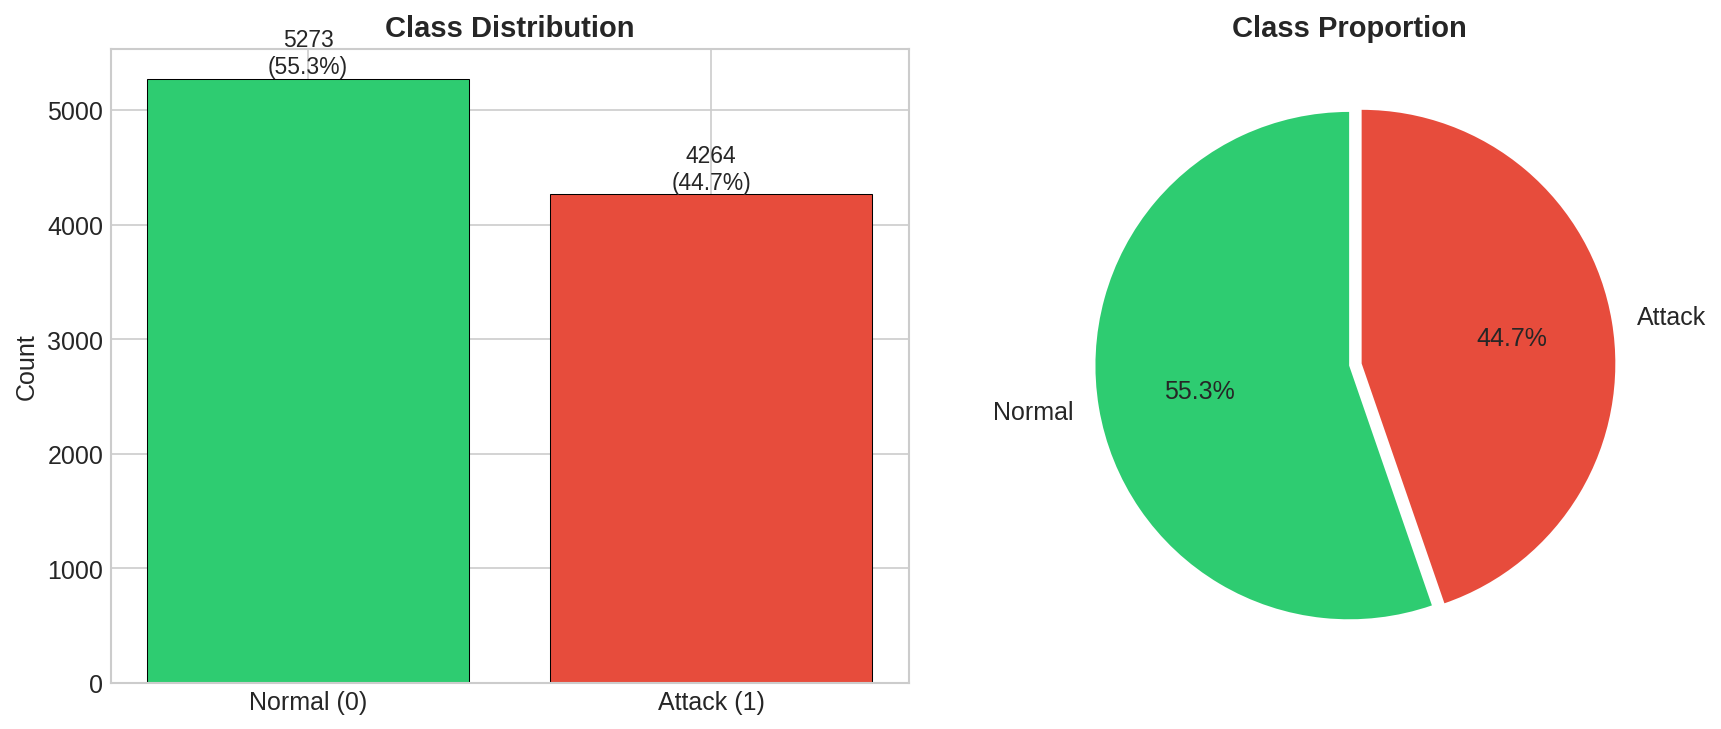
\includegraphics{figures/01_target_distribution.png}
\caption{Target distribution. The dataset is moderately imbalanced
(Normal 55.3 \% vs Attack 44.7 \%), so we did not use SMOTE.}
\end{figure}

The two classes sit at \textbf{Normal 5 273 (55.3 \%)} and
\textbf{Attack 4 264 (44.7 \%)}, a ratio of 1.24:1. Real intrusion data
in production would be closer to 99:1, but this ``balanced for
teaching'' distribution had one concrete consequence for us: we did not
apply SMOTE. The class imbalance was not pathological, and synthetic
samples would only have added noise. Instead we set
\texttt{class\_weight="balanced"} on Logistic Regression and Random
Forest, and \texttt{scale\_pos\_weight\ =\ 1.24} on XGBoost. The DNN was
trained without re-weighting and its probability outputs were calibrated
enough that no correction was needed.

\subsection{Numerical features per class (Figures 2 and
3)}\label{numerical-features-per-class-figures-2-and-3}

\begin{figure}
\centering
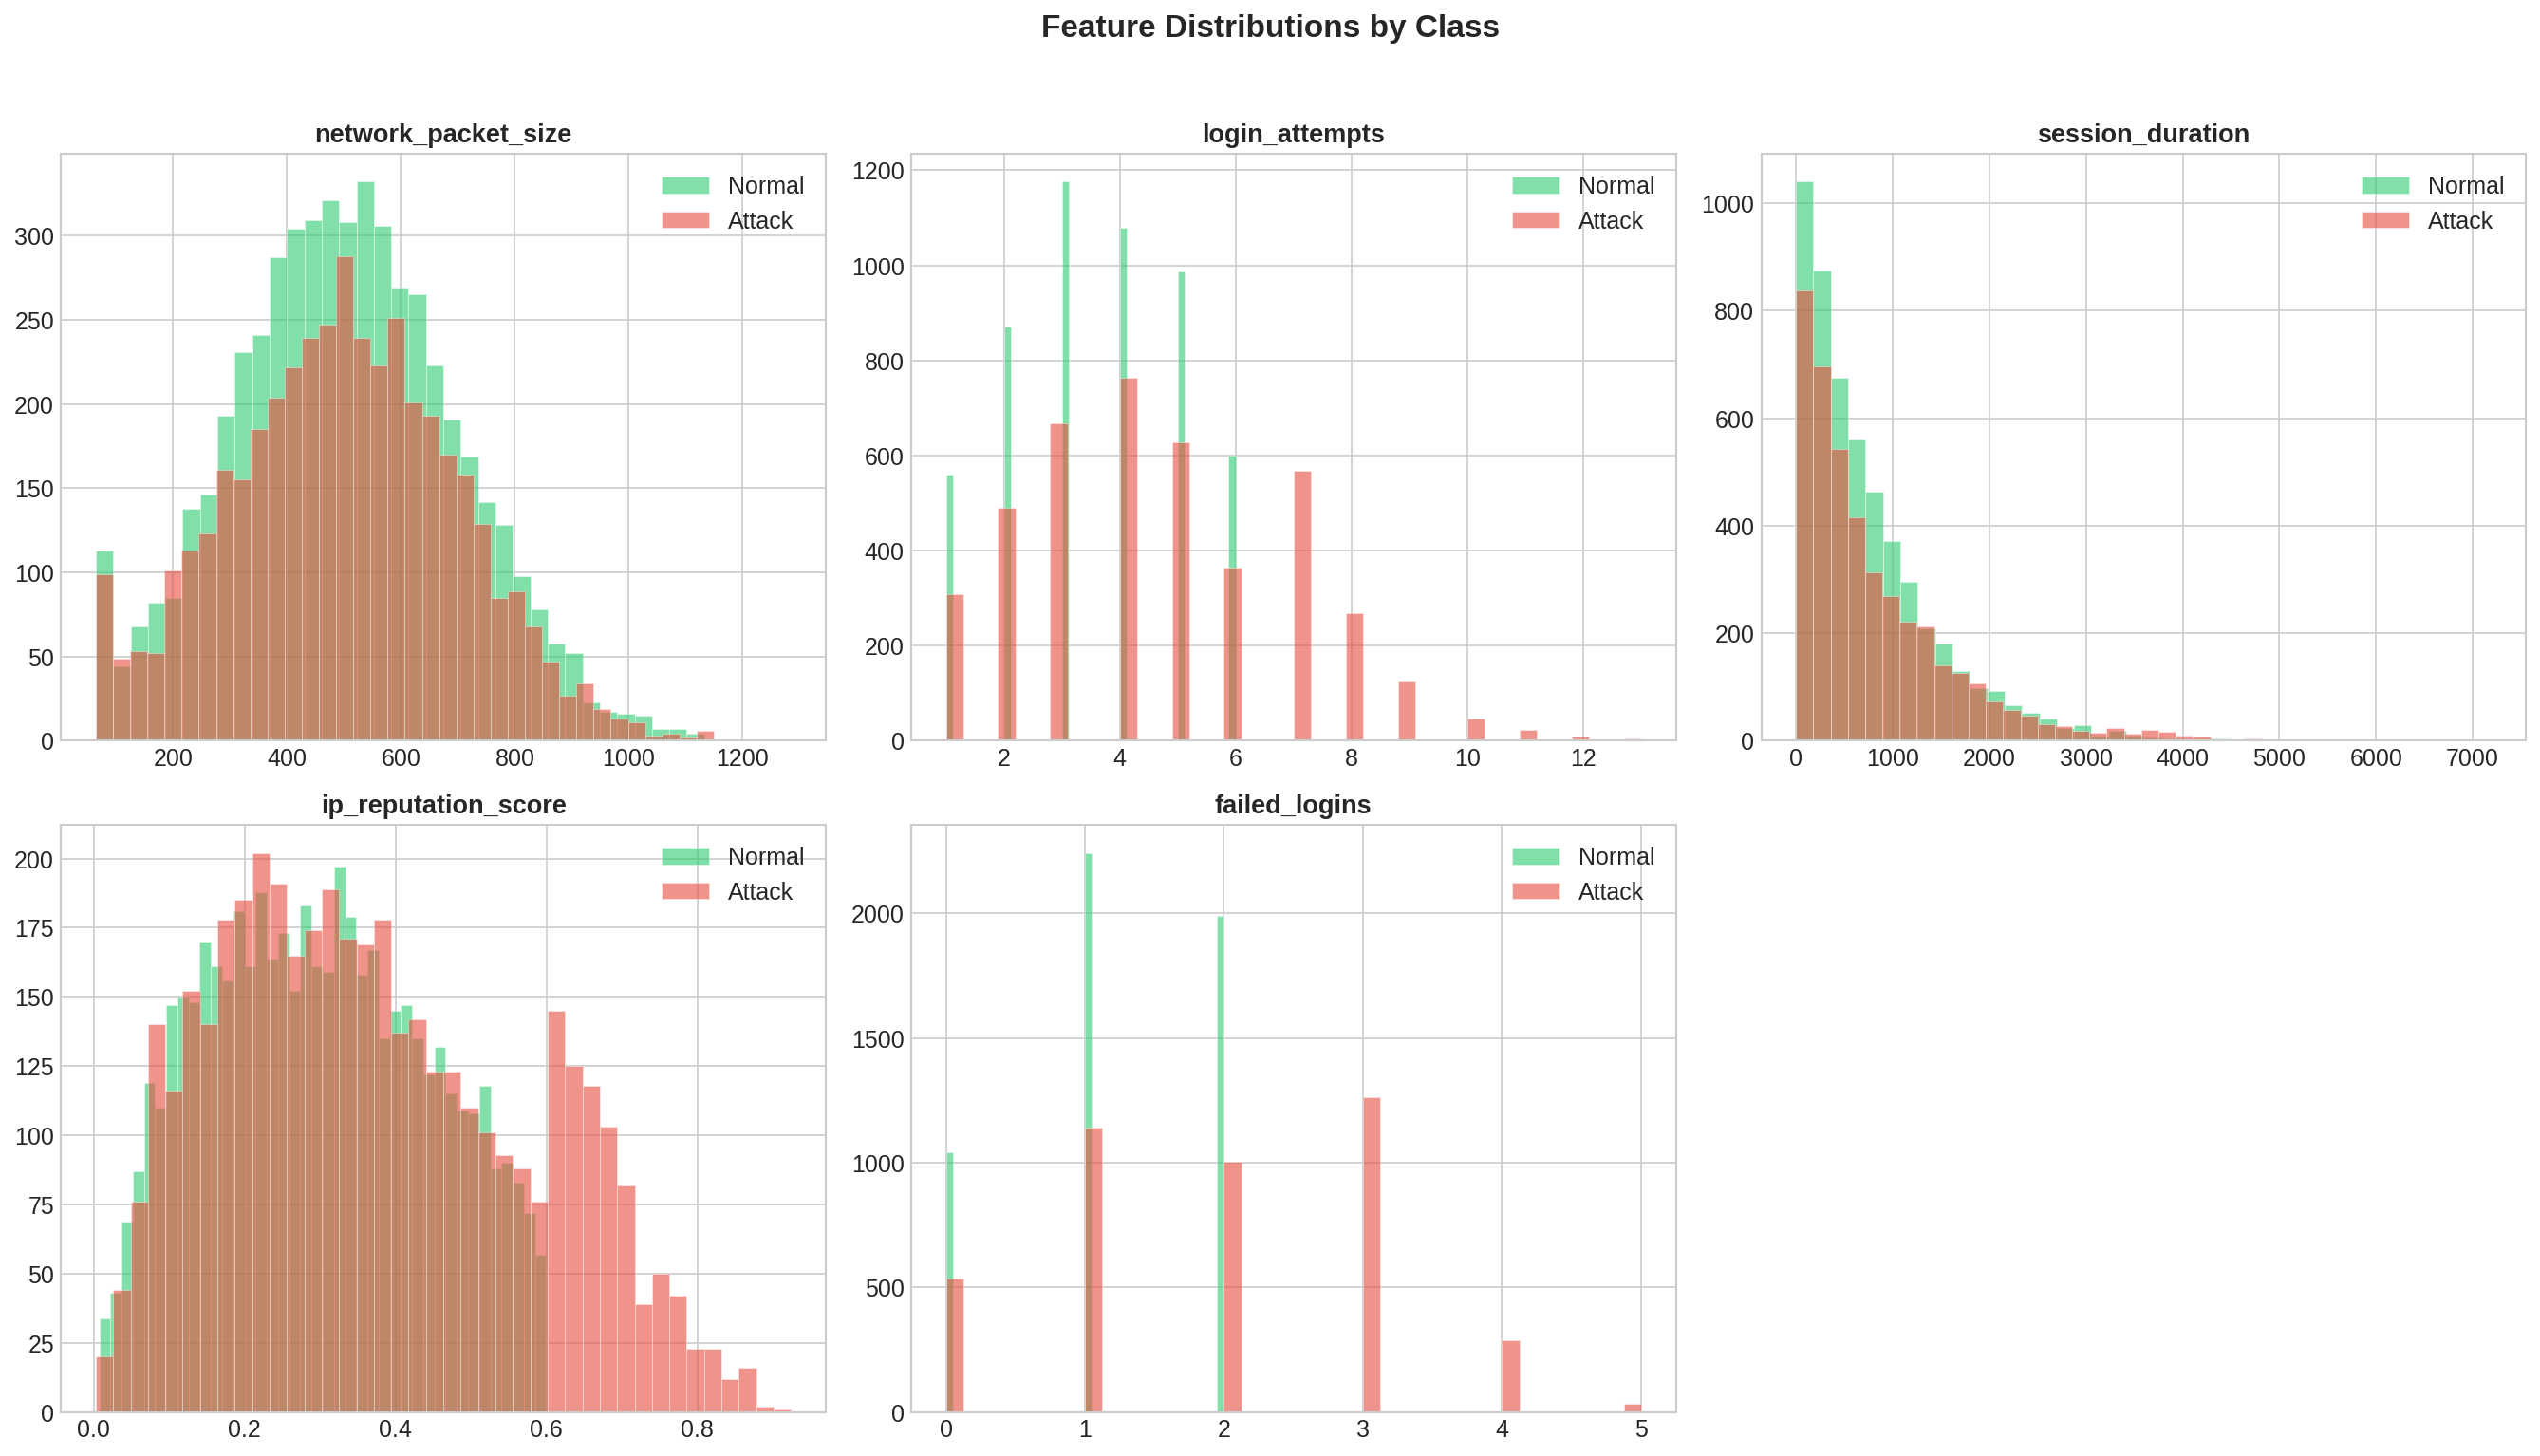
\includegraphics{figures/02_numerical_distributions.png}
\caption{Overlaid histograms of the five numerical features, split by
class. Only failed\_logins and ip\_reputation\_score visibly separate
the two classes.}
\end{figure}

\begin{figure}
\centering
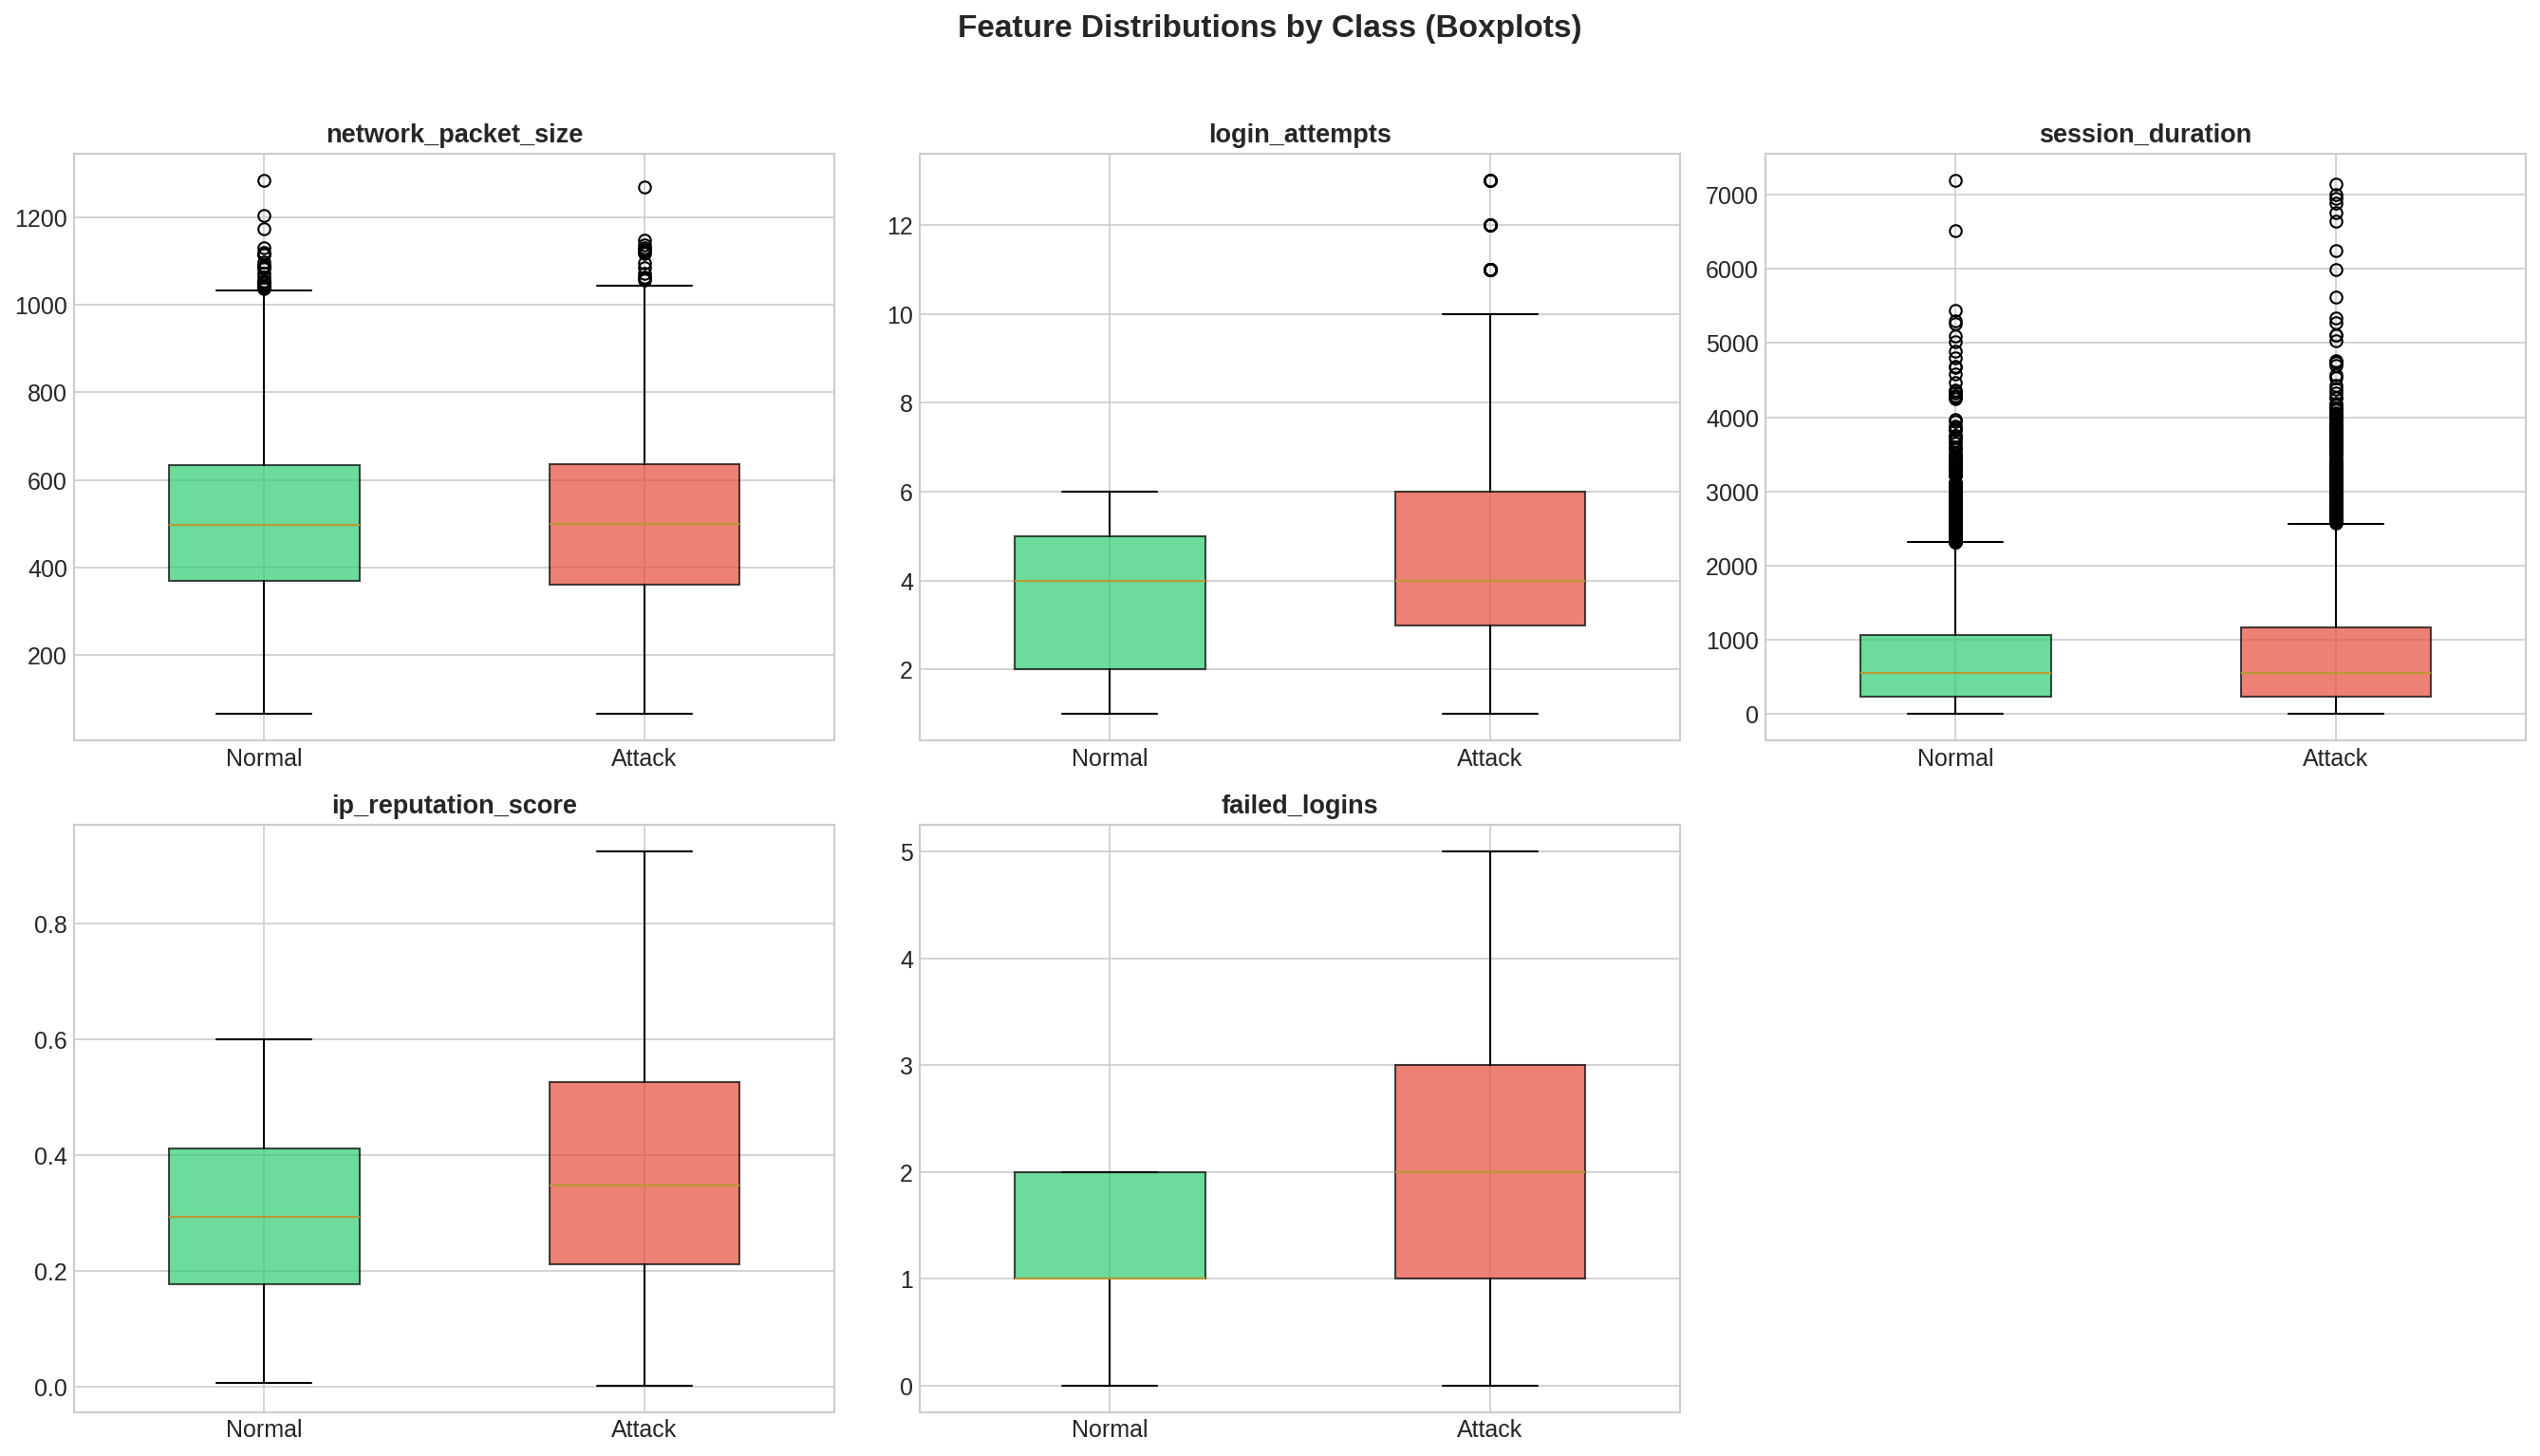
\includegraphics{figures/03_boxplots_by_class.png}
\caption{Boxplots of the same five features per class. The previous
insight is confirmed: failed\_logins and ip\_reputation\_score are the
only two numerical features with meaningfully different distributions
between classes.}
\end{figure}

These two figures tell a clear story. \texttt{failed\_logins} and
\texttt{ip\_reputation\_score} are the only two numerical features where
the distributions of the two classes visibly diverge.
\texttt{network\_packet\_size} and \texttt{session\_duration} are
essentially overlapping between classes, which is what motivated the
engineered \texttt{packet\_rate} feature in Section 2.6. We decided
early on that any model doing significantly better than a baseline that
only used these two features would have to be extracting non-linear
interactions.

\subsection{\texorpdfstring{Categorical features and the
\texttt{browser\ =\ Unknown} finding (Figure
4)}{Categorical features and the browser = Unknown finding (Figure 4)}}\label{categorical-features-and-the-browser-unknown-finding-figure-4}

\begin{figure}
\centering
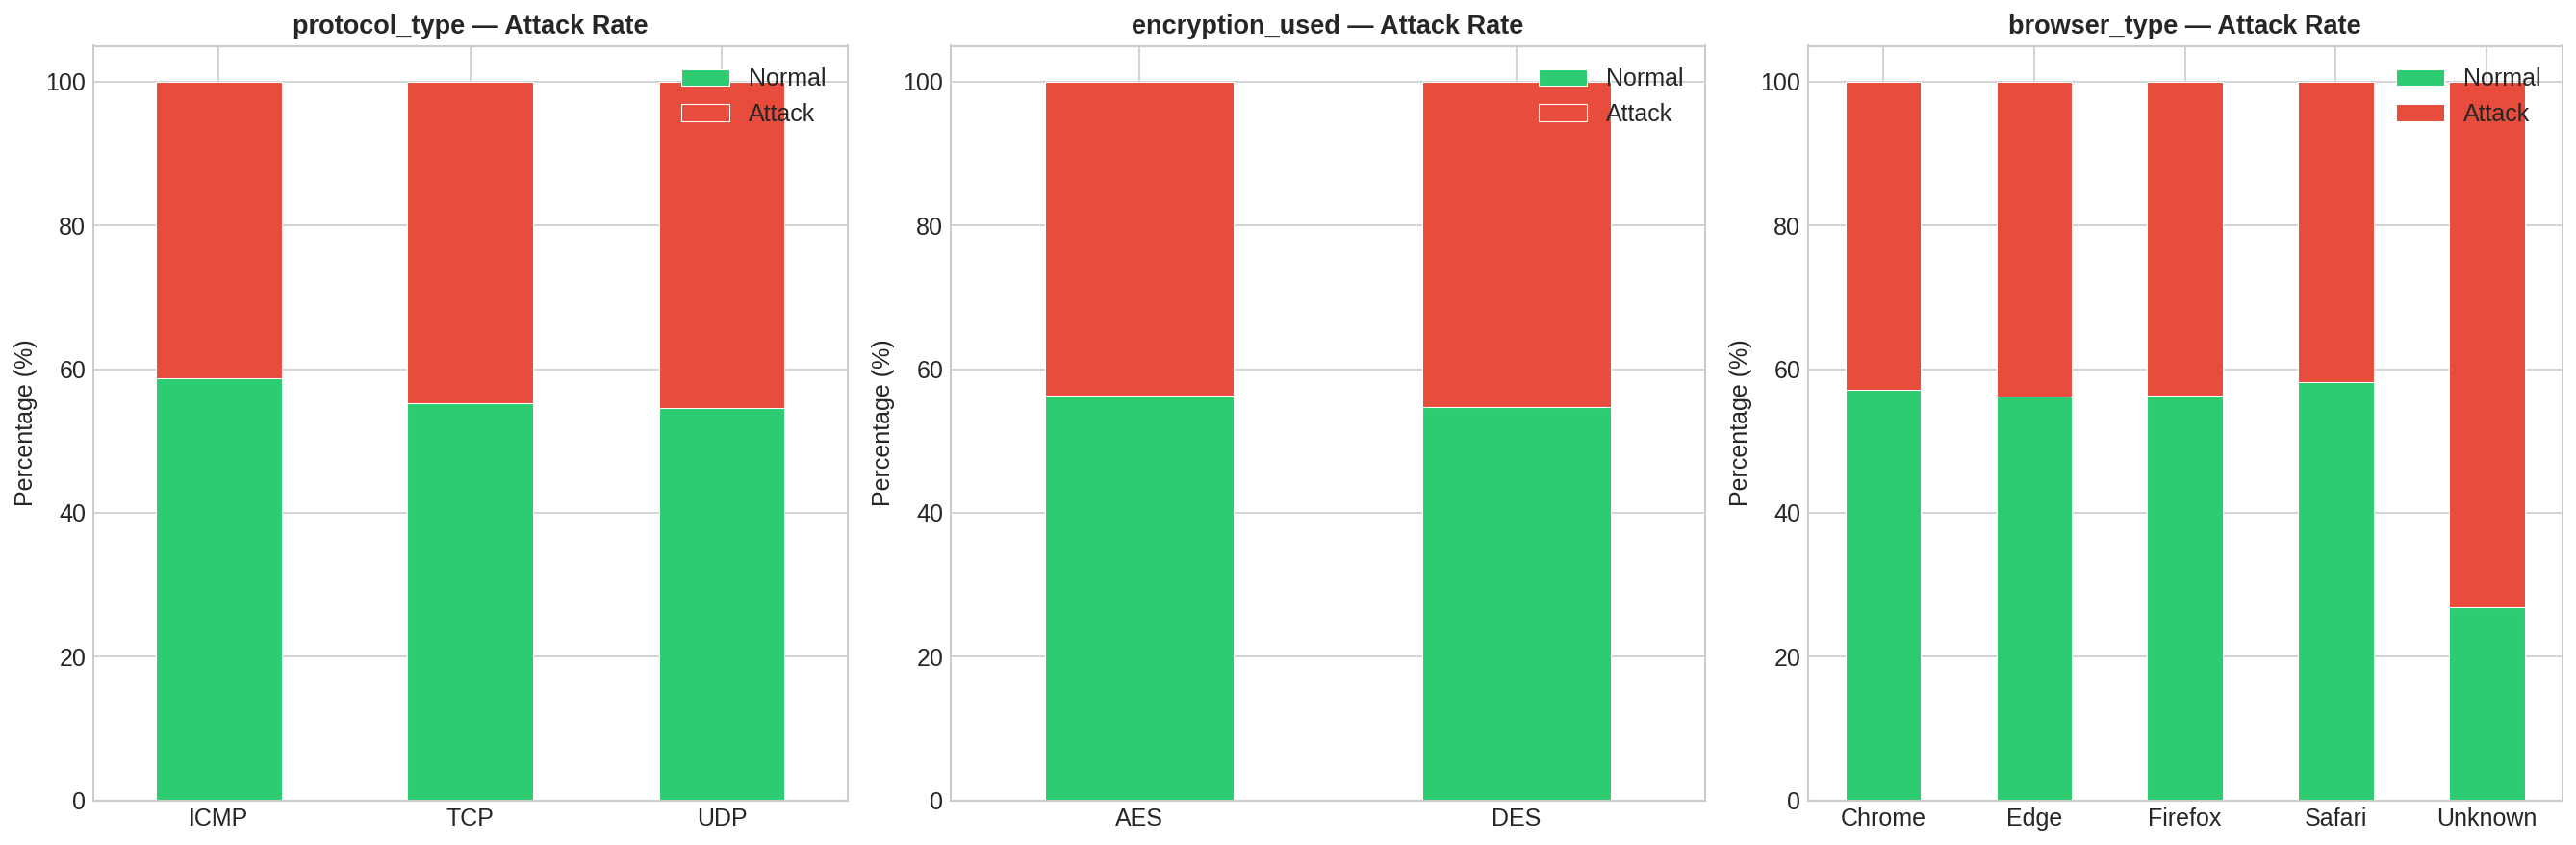
\includegraphics{figures/04_categorical_attack_rate.png}
\caption{Attack rate per modality for protocol\_type, encryption\_used
and browser\_type. The striking finding is browser\_type = Unknown
reaching 73 \% attack rate, versus 42 to 44 \% for the four known
browsers.}
\end{figure}

This figure is the single most interesting result of the EDA phase.
Protocol and encryption choices carry essentially no signal on their own
(41 to 46 \% attack rate across modalities). But
\texttt{browser\_type\ =\ Unknown}, which in practice covers bots,
\texttt{curl}, scripts, and anything that does not present a recognised
User-Agent, has a \textbf{73 \% attack rate}. That is close to 1.7× the
baseline.

We kept Unknown as a separate one-hot category rather than bucketing it
with ``Other''. Later in the SHAP analysis we confirmed that
\texttt{browser\_Unknown} was consistently in the top features every
tree-based model relied on. This was the most actionable finding from
the EDA.

\subsection{Correlation structure (Figures 5 and
6)}\label{correlation-structure-figures-5-and-6}

\begin{figure}
\centering
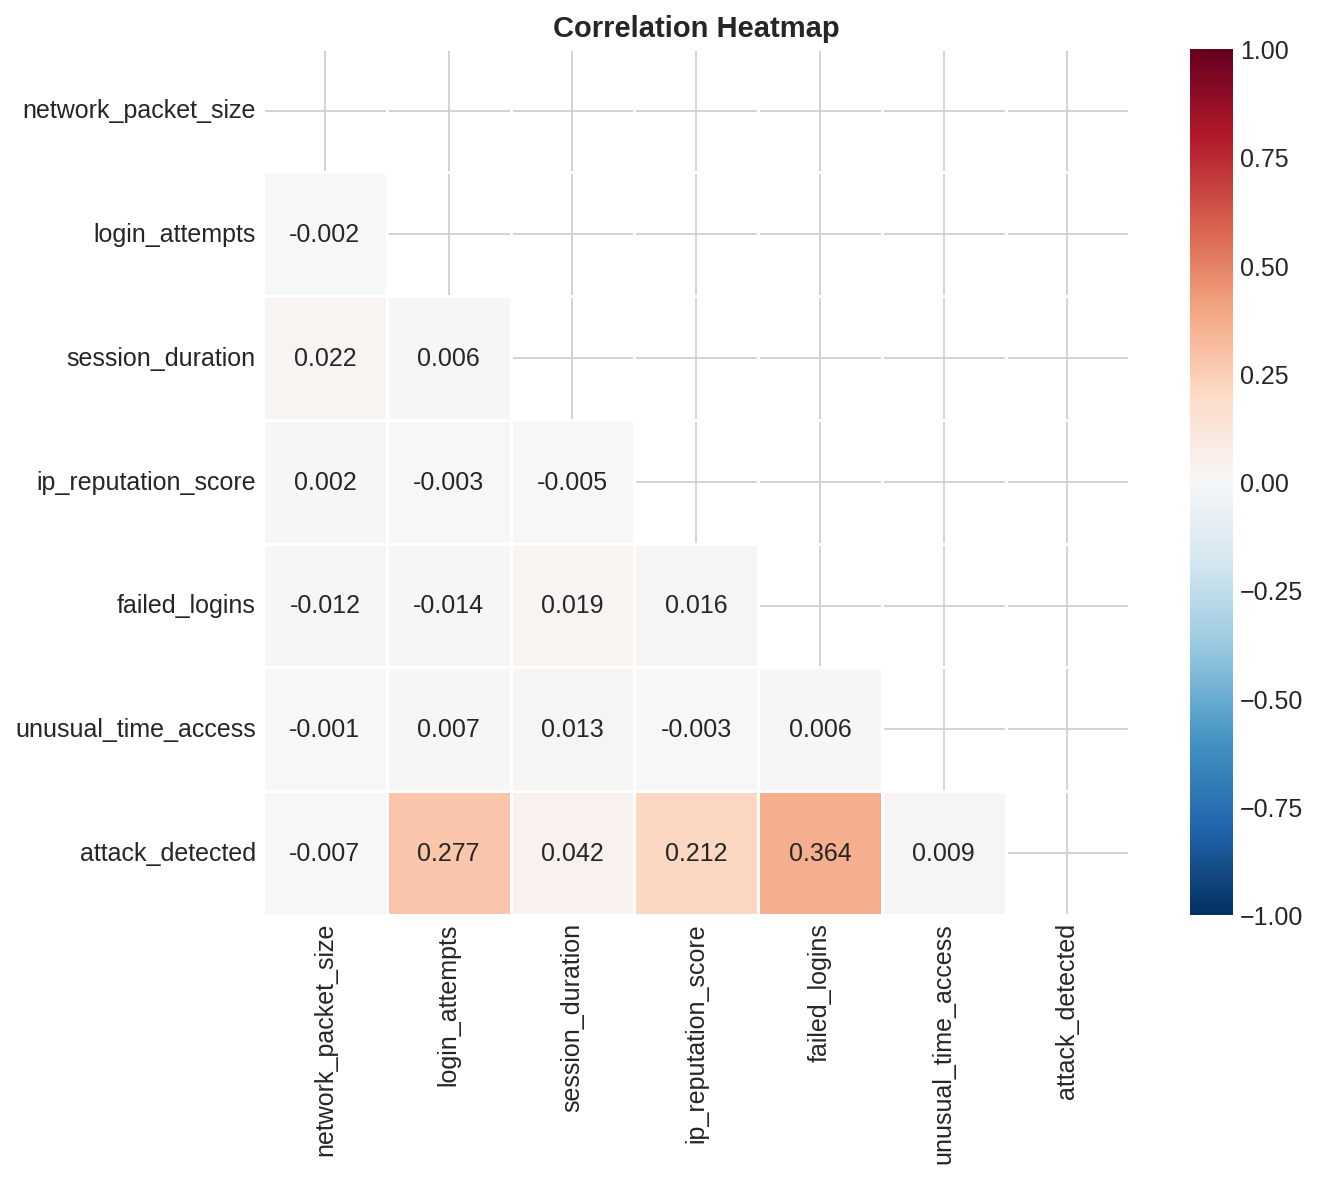
\includegraphics{figures/05_correlation_heatmap.png}
\caption{Pearson correlation heatmap. All feature-feature correlations
stay within ±0.02 (the features are mutually independent). With the
target, failed\_logins (+0.36), login\_attempts (+0.28) and
ip\_reputation\_score (+0.21) are the only non-trivial signals.}
\end{figure}

\begin{figure}
\centering
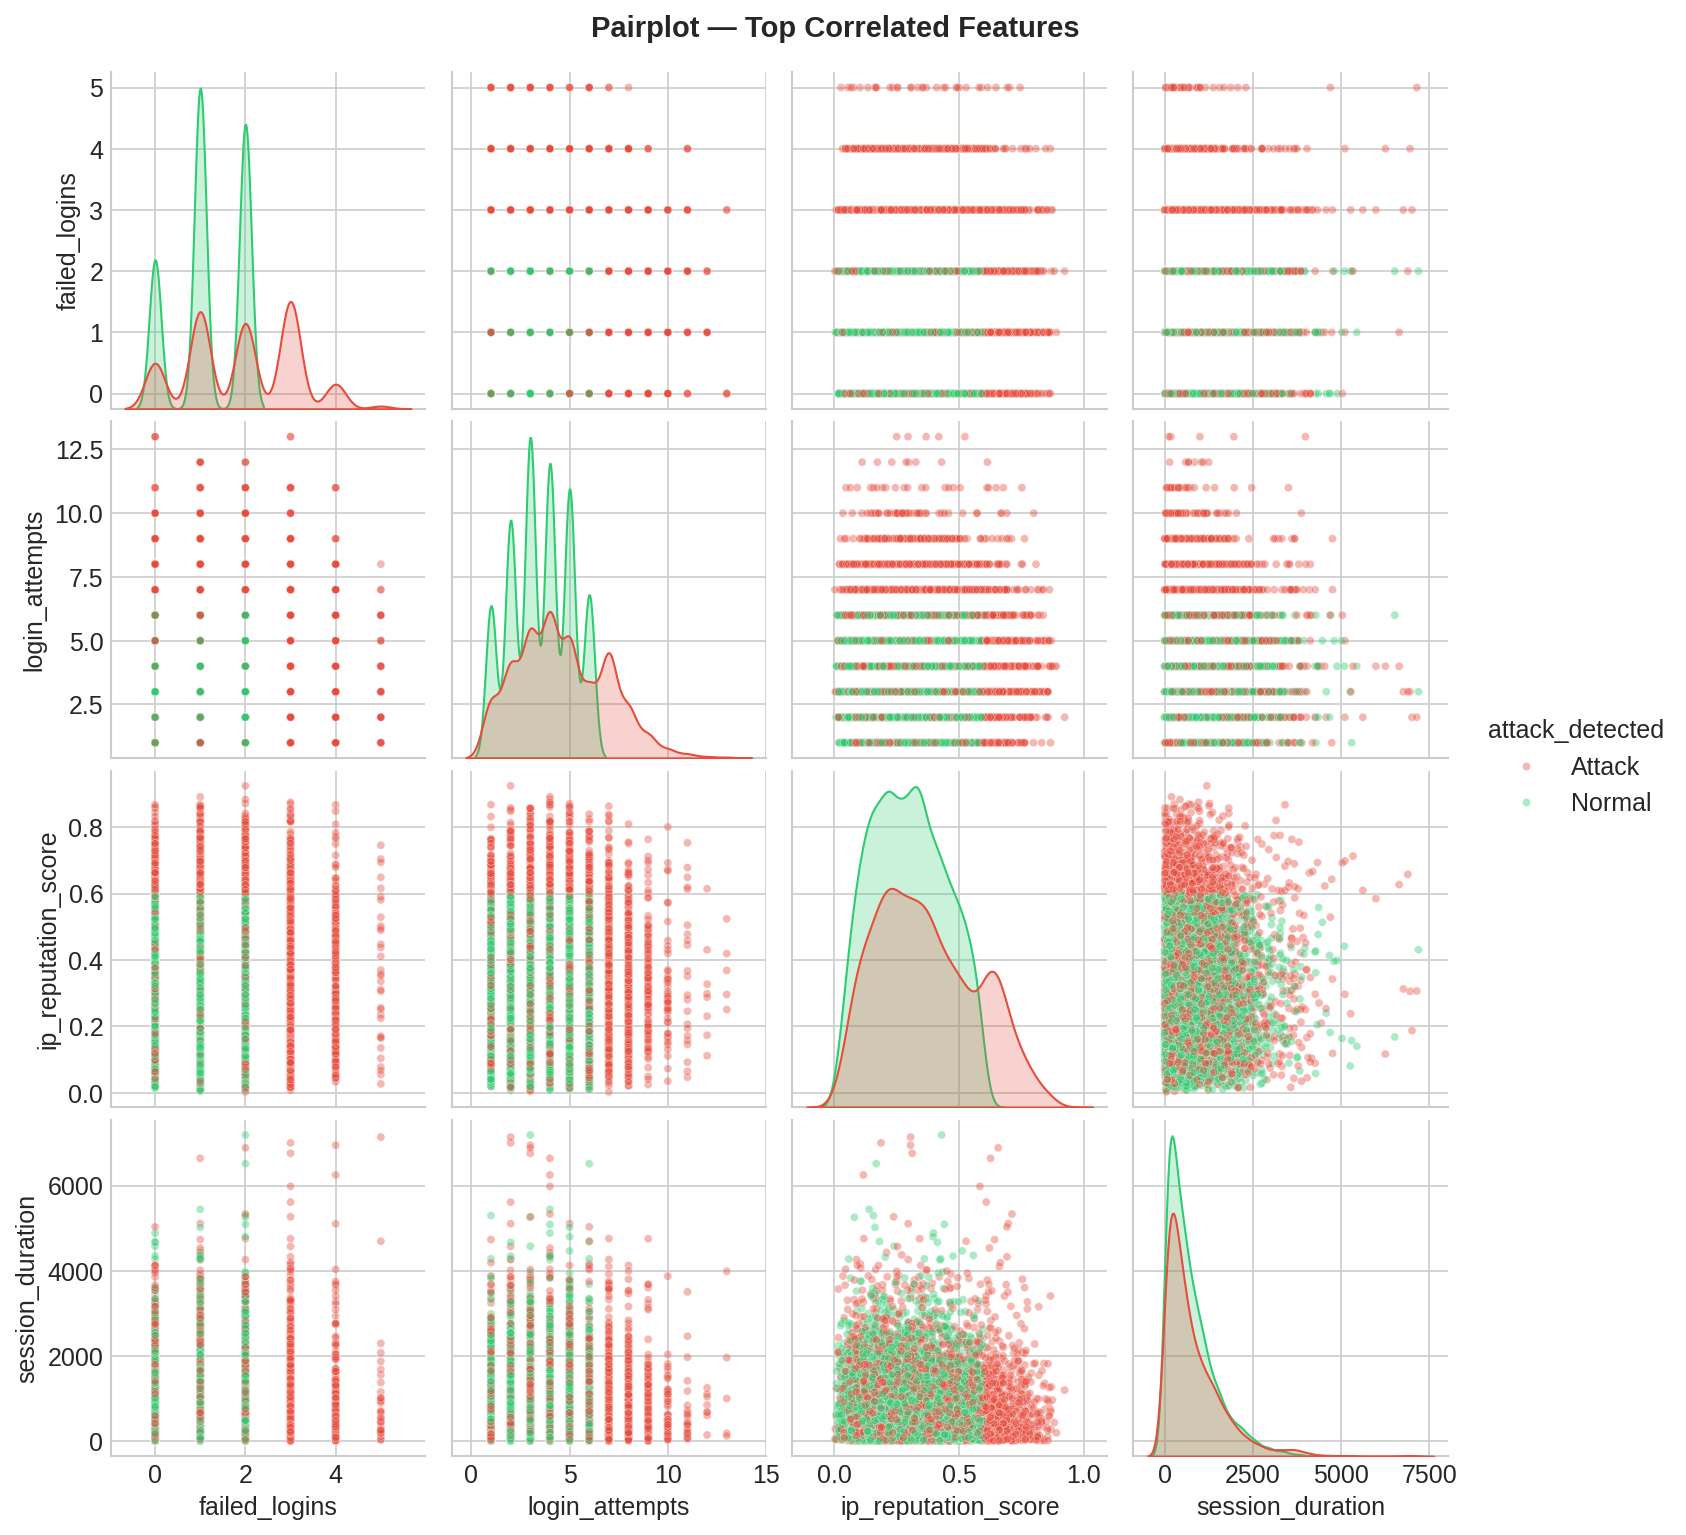
\includegraphics{figures/06_pairplot_top_features.png}
\caption{Pairplot of the four strongest predictors (login\_attempts,
failed\_logins, ip\_reputation\_score, risk\_score). The class clusters
overlap heavily in every 2D projection. The separation is inherently
non-linear in the full feature space.}
\end{figure}

Two things mattered here:

\begin{itemize}
\tightlist
\item
  \textbf{No multi-collinearity.} All inter-feature correlations are
  within ±0.02, so we did not need to drop redundant features or use
  PCA. We could feed the full set to every model and let each one decide
  what to use.
\item
  \textbf{Non-linear decision boundary.} The pairplot shows the two
  classes inter-mixed in every 2D projection. This is also why a
  Logistic Regression, even with \texttt{class\_weight="balanced"},
  plateaus at F1 = 0.73, while tree ensembles climb to 0.85.
\end{itemize}

\subsection{Feature engineering (Figures 7 and
8)}\label{feature-engineering-figures-7-and-8}

We created four engineered features in
\texttt{src/utils/feature\_engineering.py}:

\begin{itemize}
\tightlist
\item
  \texttt{login\_fail\_ratio\ =\ failed\_logins\ /\ login\_attempts}
  (guarded against division by zero)
\item
  \texttt{packet\_rate\ =\ network\_packet\_size\ /\ session\_duration}
  (guarded the same way)
\item
  \texttt{risk\_score\ =\ 0.4\ ·\ ip\_reputation\_score\ +\ 0.3\ ·\ unusual\_time\_access\ +\ 0.3\ ·\ login\_fail\_ratio}
\item
  \texttt{high\_risk\_ip\ =\ (ip\_reputation\_score\ \textgreater{}\ 0.7)}
  as an integer flag
\end{itemize}

\begin{figure}
\centering
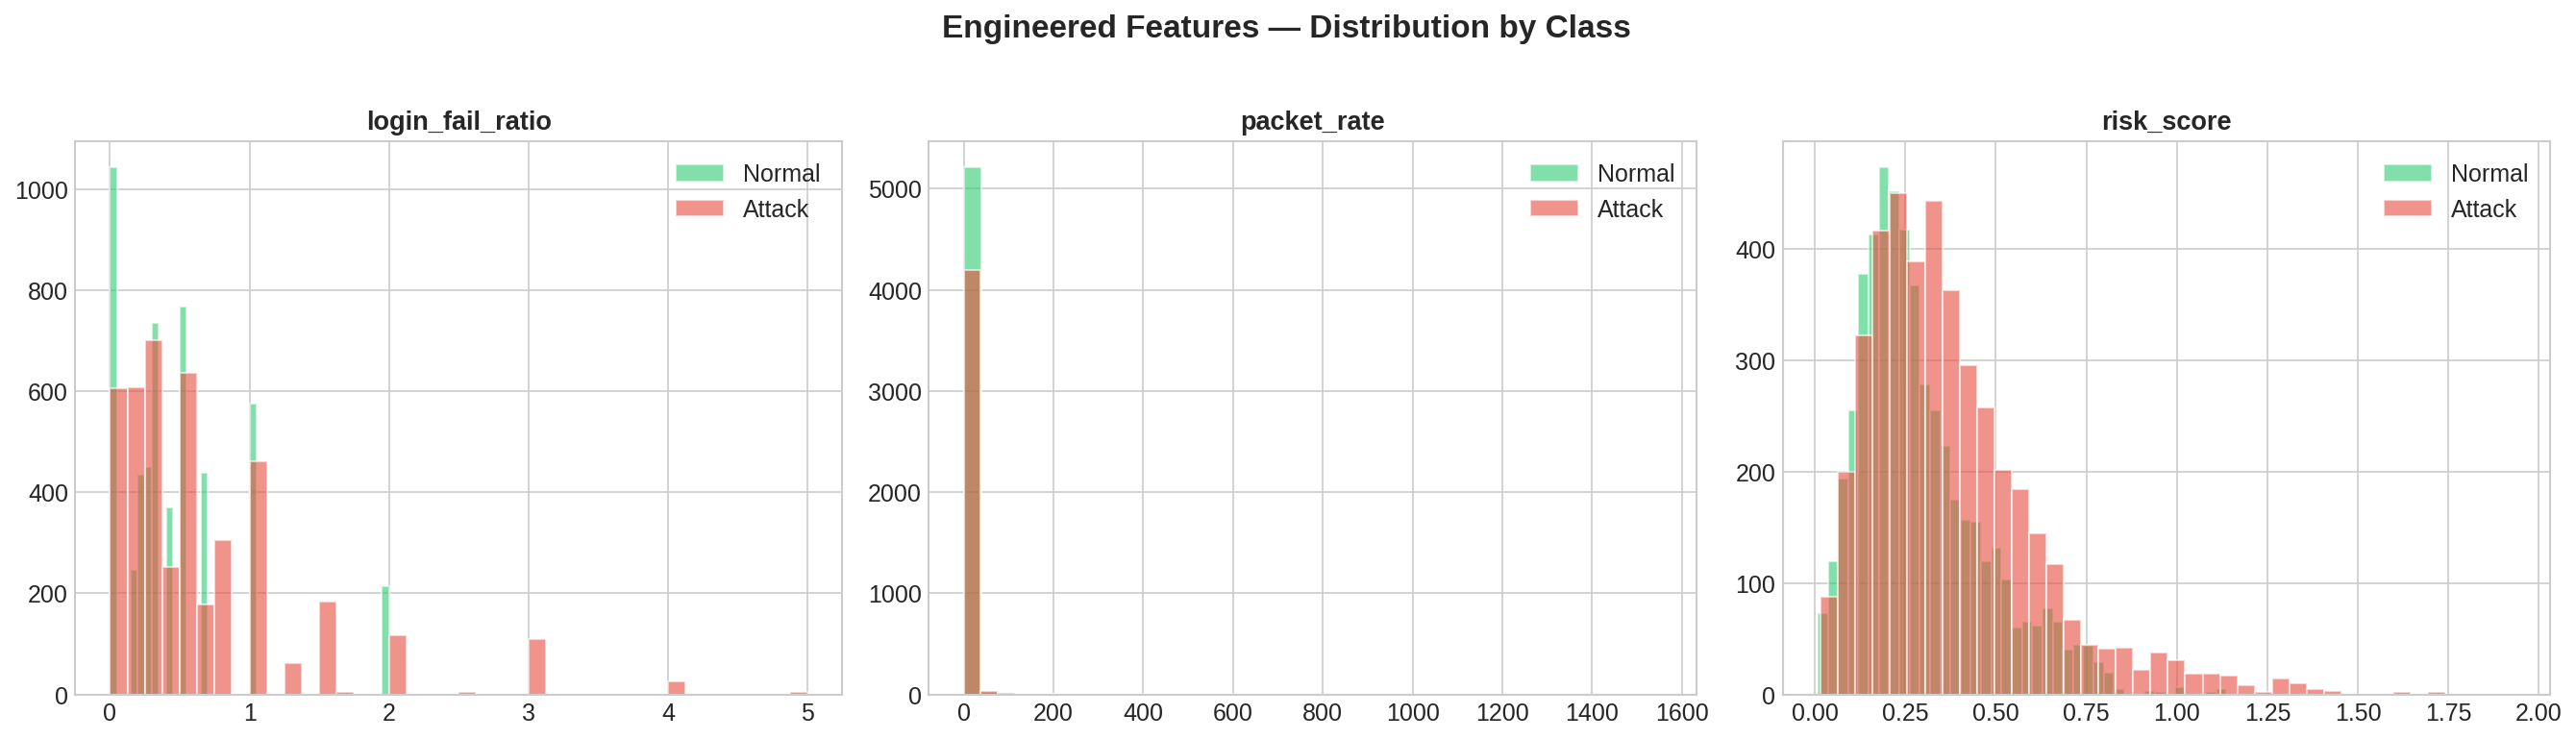
\includegraphics{figures/07_engineered_features.png}
\caption{Distributions of the three numerical engineered features per
class. login\_fail\_ratio cleanly separates the classes above ratio
\textasciitilde{} 1; risk\_score adds a modest but meaningful signal;
packet\_rate is essentially noise, confirming the EDA.}
\end{figure}

\begin{figure}
\centering
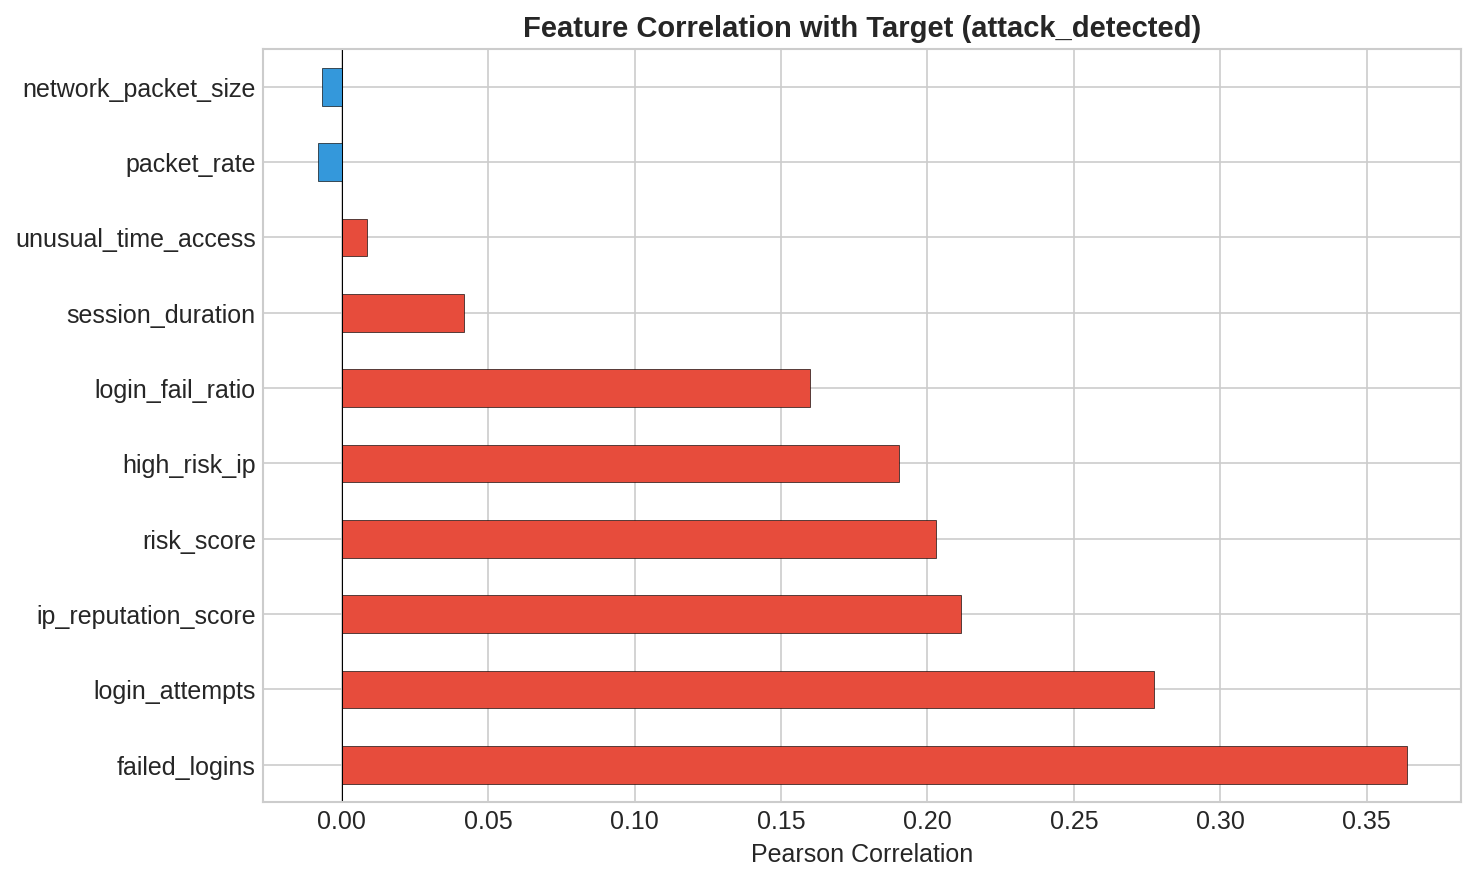
\includegraphics{figures/08_feature_importance_correlation.png}
\caption{Bar chart of Pearson correlation with the target, ranked. Three
out of four engineered features (risk\_score, high\_risk\_ip,
login\_fail\_ratio) land in the top six, validating the engineering
decisions.}
\end{figure}

The ranking in Figure 8 is what we actually used to decide what to keep.
\texttt{risk\_score}, \texttt{high\_risk\_ip}, and
\texttt{login\_fail\_ratio}, all engineered, rank 4th, 5th, and 6th
respectively, beating four of the raw features. \texttt{packet\_rate}
ranked dead last, in line with the fact that the features it combines
also have essentially zero correlation with the target. We kept it
anyway, because tree-based models can still exploit it through
interactions that univariate correlation cannot surface.

\subsection{Final preprocessing
pipeline}\label{final-preprocessing-pipeline}

The fitted pipeline, wrapped in a scikit-learn
\texttt{ColumnTransformer}, is:

\begin{itemize}
\tightlist
\item
  \textbf{Numerical} (5 raw + 3 engineered = 8 features):
  \texttt{StandardScaler} (Z-Score)
\item
  \textbf{Categorical} (\texttt{protocol\_type},
  \texttt{encryption\_used}, \texttt{browser\_type}):
  \texttt{OneHotEncoder(drop="first",\ handle\_unknown="ignore")}. The
  \texttt{handle\_unknown="ignore"} lets inference-time Unknown values
  encode as all zeros rather than throw.
\item
  \textbf{Binary} (\texttt{unusual\_time\_access} and
  \texttt{high\_risk\_ip}): pass-through
\end{itemize}

After the transformer, each session is an 18-column vector. We split
80/20 stratified on the target, which gave us
\texttt{X\_train.shape\ =\ (7629,\ 18)} and
\texttt{X\_test.shape\ =\ (1908,\ 18)}. The random seed (42) is fixed in
\texttt{numpy}, \texttt{scikit-learn} and \texttt{tensorflow} for exact
reproducibility.

The entire pipeline is serialised to
\texttt{saved\_models/preprocessor.joblib}, so training and inference
use the \emph{same} transformer. This avoids training-serving skew by
construction.

\begin{center}\rule{0.5\linewidth}{0.5pt}\end{center}

\section{Model Training and
Comparison}\label{model-training-and-comparison}

Our strategy was to build up complexity step by step. One baseline per
hypothesis, and we only moved on to the next model when the previous one
had taught us something. All runs were tracked in MLflow under the
experiment \texttt{cybersecurity-ids}.

\subsection{Classical baselines (Figures 9 and
10)}\label{classical-baselines-figures-9-and-10}

We trained four baselines:

\begin{itemize}
\tightlist
\item
  \textbf{Dummy Classifier} (\texttt{strategy="most\_frequent"}): the
  floor. It predicts Normal every time, which gives F1 = 0.0000 and
  Accuracy = 0.5529. Any model we keep must beat this.
\item
  \textbf{Logistic Regression}: tests whether the problem is linearly
  separable.
\item
  \textbf{Random Forest} (\texttt{n\_estimators=200},
  \texttt{max\_depth=15}, \texttt{class\_weight="balanced"}): tests
  whether tree ensembles capture the non-linear boundary we saw in
  Section 2.5.
\item
  \textbf{XGBoost} (\texttt{n\_estimators=200}, \texttt{max\_depth=6},
  \texttt{learning\_rate=0.1}, \texttt{scale\_pos\_weight=1.24}): tests
  whether gradient boosting adds anything over bagging.
\end{itemize}

All four were logged to MLflow with parameters, metrics (accuracy,
precision, recall, F1, ROC-AUC, PR-AUC), train time, inference time, and
the fitted model artefact.

\begin{figure}
\centering
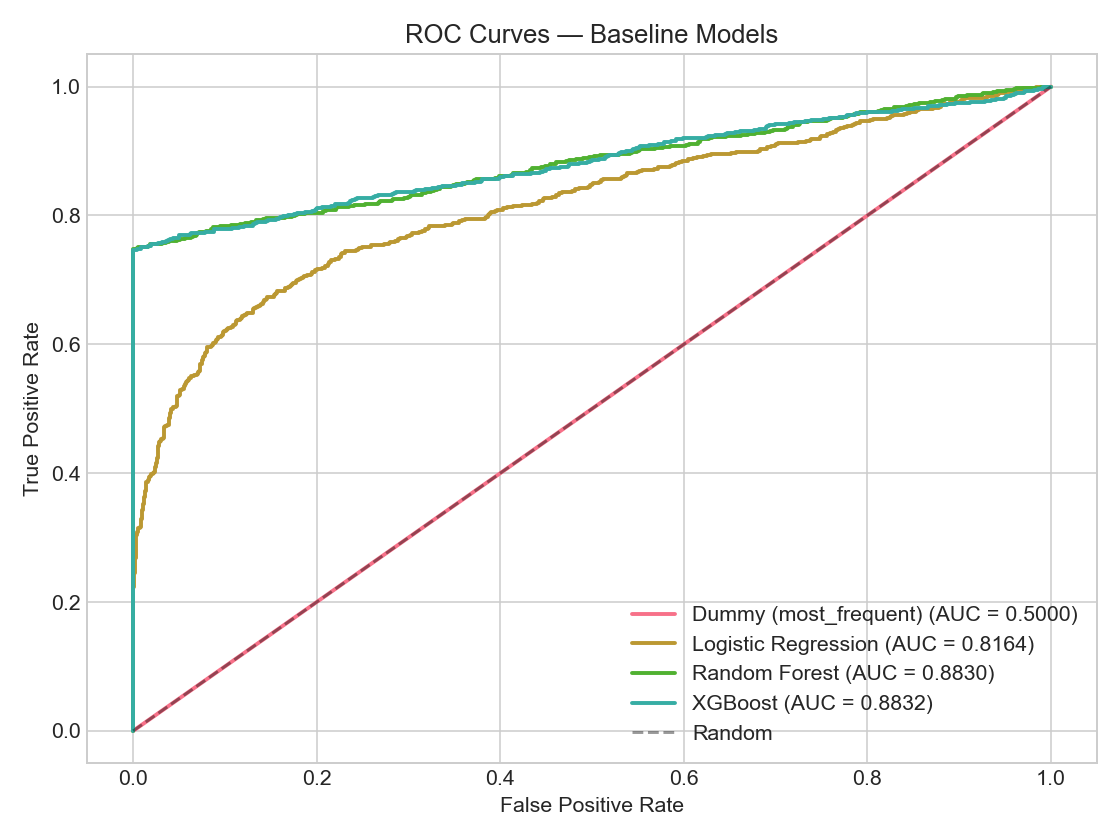
\includegraphics{figures/09_baselines_roc.png}
\caption{ROC curves of the four baselines on the test set. Random Forest
and XGBoost lie almost on top of each other at AUC \textasciitilde{}
0.88.}
\end{figure}

\begin{figure}
\centering
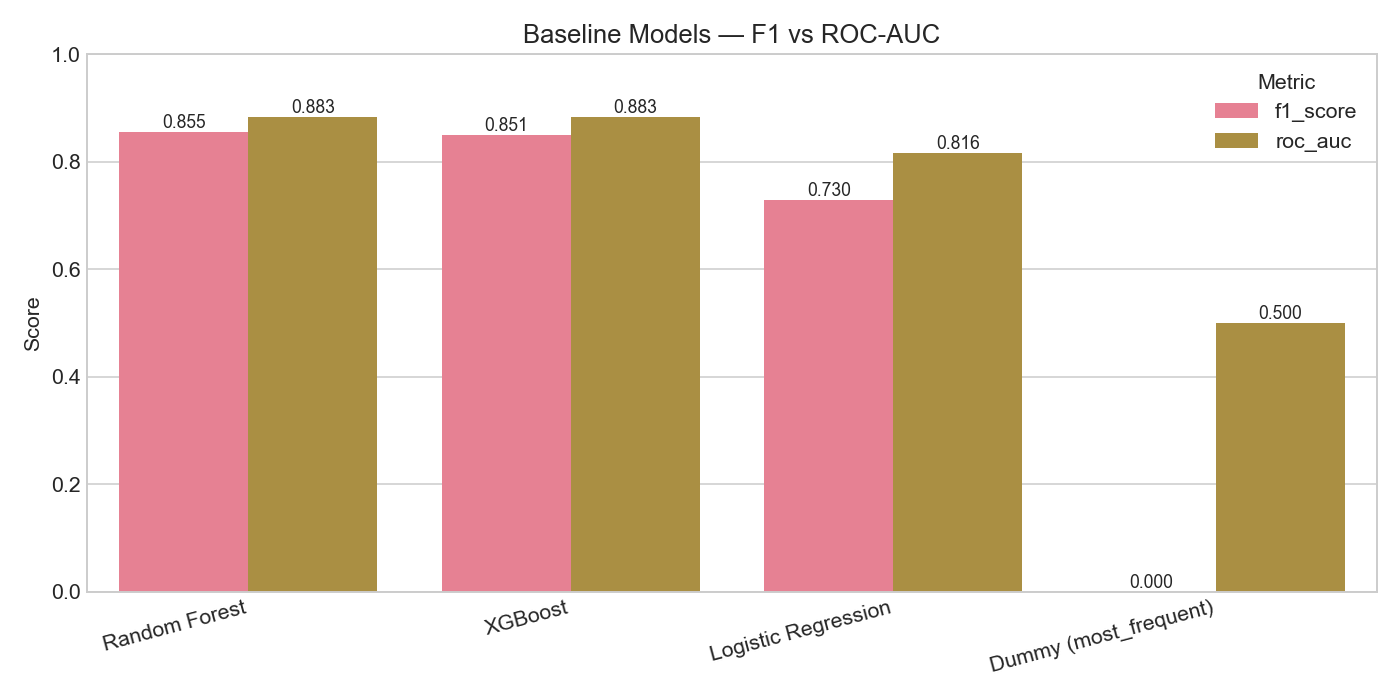
\includegraphics{figures/10_baselines_comparison.png}
\caption{Barplot comparison of F1 vs AUC for the four baselines. Random
Forest wins F1 (0.855); XGBoost wins AUC by a hair (0.8832 vs 0.8830).}
\end{figure}

The measured results on the held-out test set (1908 samples):

\begin{longtable}[]{@{}
  >{\raggedright\arraybackslash}p{(\columnwidth - 10\tabcolsep) * \real{0.3472}}
  >{\raggedleft\arraybackslash}p{(\columnwidth - 10\tabcolsep) * \real{0.1389}}
  >{\raggedleft\arraybackslash}p{(\columnwidth - 10\tabcolsep) * \real{0.1111}}
  >{\raggedleft\arraybackslash}p{(\columnwidth - 10\tabcolsep) * \real{0.1250}}
  >{\raggedleft\arraybackslash}p{(\columnwidth - 10\tabcolsep) * \real{0.1250}}
  >{\raggedleft\arraybackslash}p{(\columnwidth - 10\tabcolsep) * \real{0.1528}}@{}}
\toprule\noalign{}
\begin{minipage}[b]{\linewidth}\raggedright
Model
\end{minipage} & \begin{minipage}[b]{\linewidth}\raggedleft
Accuracy
\end{minipage} & \begin{minipage}[b]{\linewidth}\raggedleft
F1
\end{minipage} & \begin{minipage}[b]{\linewidth}\raggedleft
ROC-AUC
\end{minipage} & \begin{minipage}[b]{\linewidth}\raggedleft
Train
\end{minipage} & \begin{minipage}[b]{\linewidth}\raggedleft
Inference
\end{minipage} \\
\midrule\noalign{}
\endhead
\bottomrule\noalign{}
\endlastfoot
Dummy (most\_frequent) & 0.5529 & 0.0000 & 0.5000 & 0.00 s & 4.1 ms \\
Logistic Regression & 0.7573 & 0.7297 & 0.8164 & 0.02 s & 0.2 ms \\
\textbf{Random Forest} & 0.8868 & \textbf{0.8550} & 0.8830 & 0.41 s &
67.8 ms \\
XGBoost & 0.8826 & 0.8507 & \textbf{0.8832} & 0.25 s & 1.8 ms \\
\end{longtable}

Three findings came out of this step:

\begin{itemize}
\tightlist
\item
  The Logistic Regression at F1 = 0.73 is actually a useful signal.
  Three linear features (\texttt{failed\_logins},
  \texttt{login\_attempts}, \texttt{ip\_reputation\_score}) already
  carry most of what is there. Our non-linear models had to do the other
  \textasciitilde12 points of F1.
\item
  Random Forest and XGBoost are effectively tied. RF edges F1 by 0.004
  and XGBoost edges AUC by 0.0002. We picked RF as the baseline champion
  on the F1 tie-break, but kept evaluating both through the rest of the
  project.
\item
  \textbf{Precision on Attack is 1.00 for Random Forest}: zero false
  positives on the test set. Recall sits at 0.75, meaning we miss about
  a quarter of the attacks. This recall ceiling will recur across every
  model, and we discuss it as a property of the feature set, not of the
  algorithm.
\end{itemize}

\subsection{Deep Learning (Figures 11 and
12)}\label{deep-learning-figures-11-and-12}

We trained four DNN variants with Keras, all from the same parametric
builder in \texttt{src/models/deep\_learning.py}:

\begin{itemize}
\tightlist
\item
  \textbf{Baseline:}
  \texttt{Dense(128)\ →\ Dropout(0.3)\ →\ Dense(64)\ →\ Dropout(0.3)\ →\ Dense(32)\ →\ Dense(1,\ sigmoid)},
  Adam (lr=1e-3), binary cross-entropy, \texttt{batch\_size=32},
  \texttt{validation\_split=0.15}.
\item
  \textbf{v1:} same architecture, \texttt{dropout\ =\ 0.5} (stronger
  regularisation).
\item
  \textbf{v2:} same architecture, \texttt{batch\_size\ =\ 128} (faster
  convergence).
\item
  \textbf{v3:} deeper architecture \texttt{256\ →\ 128\ →\ 64\ →\ 32},
  \texttt{dropout\ =\ 0.3}, \texttt{batch\_size\ =\ 32}.
\end{itemize}

Every variant used
\texttt{EarlyStopping(patience=10,\ restore\_best\_weights=True)} and
\texttt{ReduceLROnPlateau(factor=0.5,\ patience=5)}. All four were
logged to MLflow alongside the baselines so we could compare them side
by side.

\begin{figure}
\centering
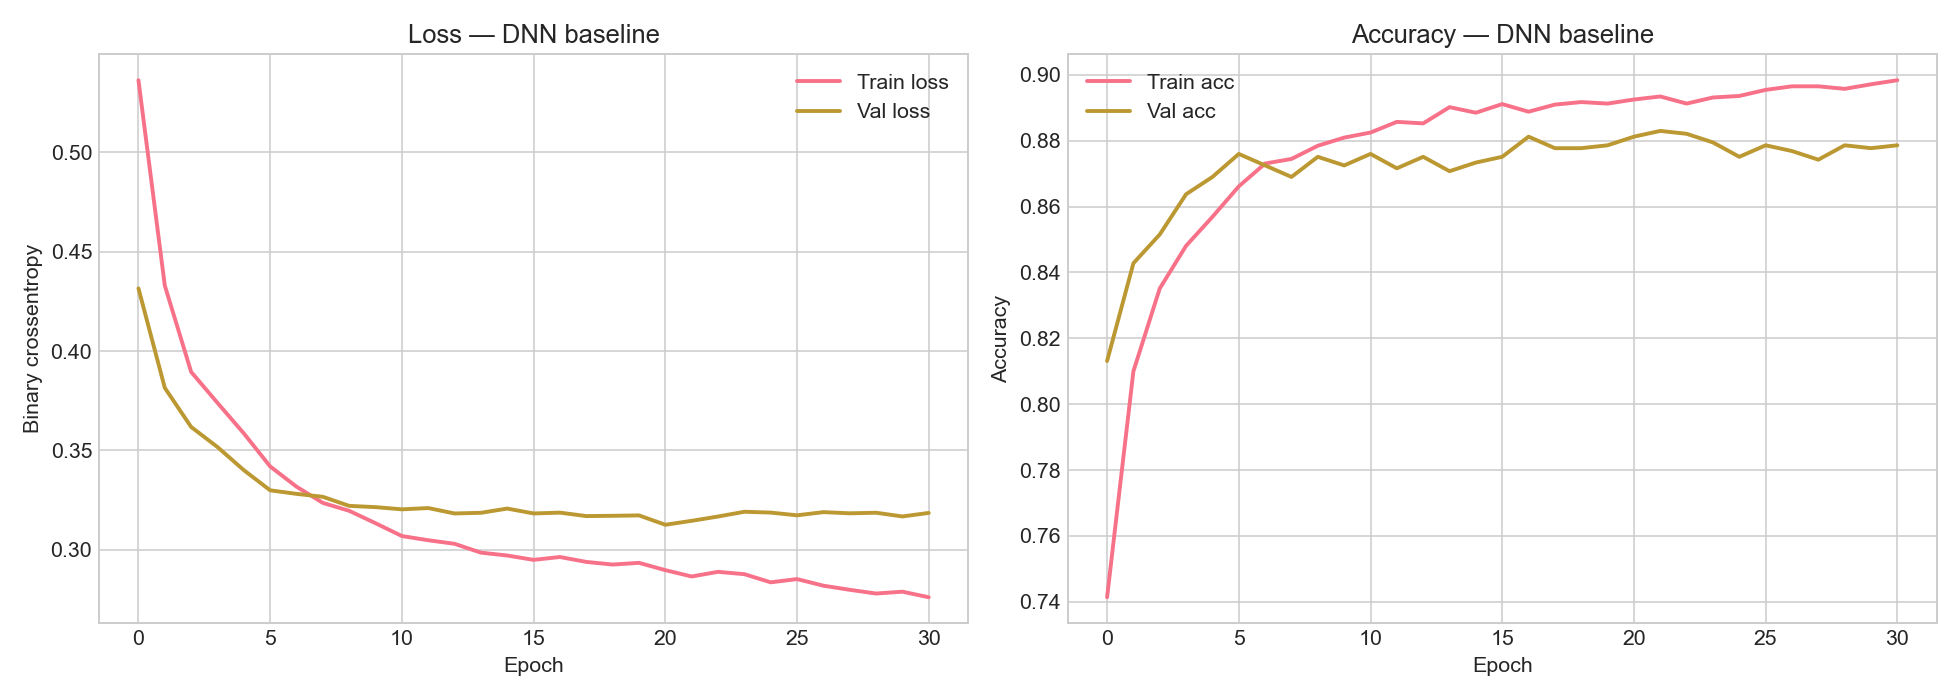
\includegraphics{figures/11_dnn_baseline_learning_curves.png}
\caption{DNN baseline learning curves (train vs validation).
EarlyStopping restored the best weights around epoch 22, before
val\_loss started creeping up.}
\end{figure}

\begin{figure}
\centering
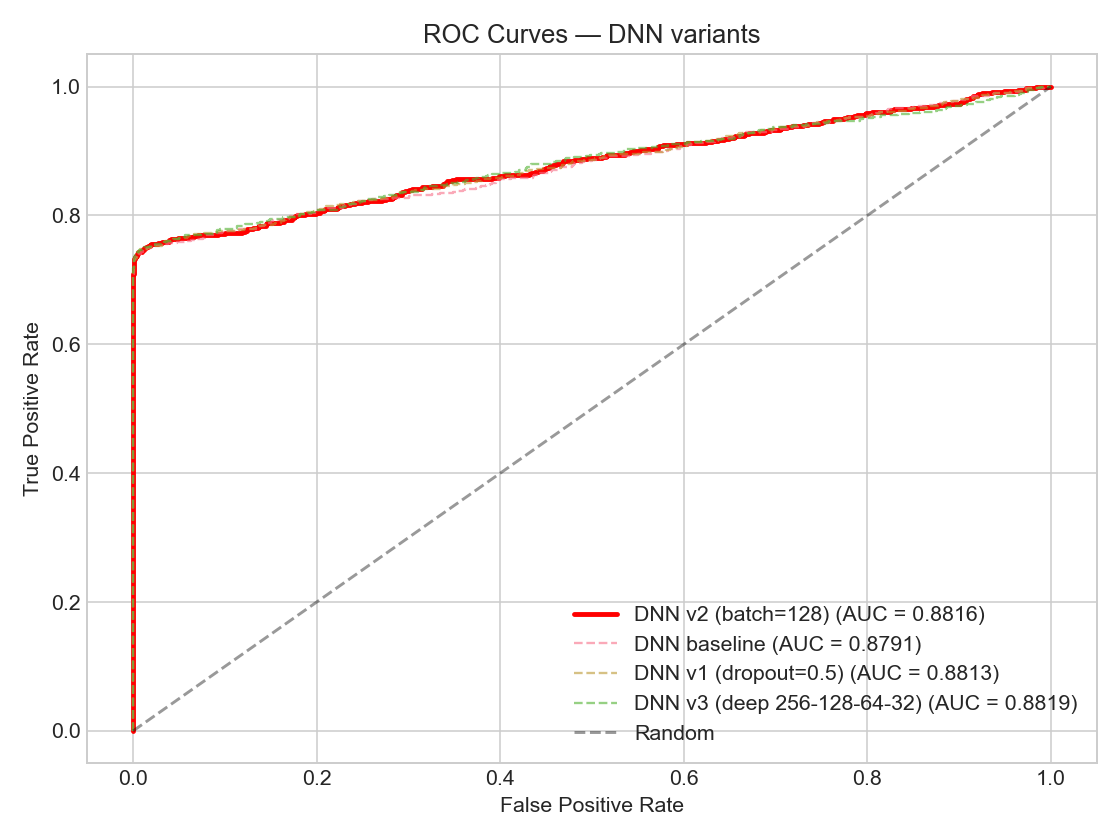
\includegraphics{figures/12_dnn_variants_roc.png}
\caption{ROC curves for the four DNN variants. All four sit within a
0.003 AUC band, well inside the region Random Forest already occupies.}
\end{figure}

Results on the test set:

\begin{longtable}[]{@{}
  >{\raggedright\arraybackslash}p{(\columnwidth - 10\tabcolsep) * \real{0.4400}}
  >{\raggedleft\arraybackslash}p{(\columnwidth - 10\tabcolsep) * \real{0.1333}}
  >{\raggedleft\arraybackslash}p{(\columnwidth - 10\tabcolsep) * \real{0.1067}}
  >{\raggedleft\arraybackslash}p{(\columnwidth - 10\tabcolsep) * \real{0.1067}}
  >{\raggedleft\arraybackslash}p{(\columnwidth - 10\tabcolsep) * \real{0.1067}}
  >{\raggedleft\arraybackslash}p{(\columnwidth - 10\tabcolsep) * \real{0.1067}}@{}}
\toprule\noalign{}
\begin{minipage}[b]{\linewidth}\raggedright
Variant
\end{minipage} & \begin{minipage}[b]{\linewidth}\raggedleft
Accuracy
\end{minipage} & \begin{minipage}[b]{\linewidth}\raggedleft
F1
\end{minipage} & \begin{minipage}[b]{\linewidth}\raggedleft
AUC
\end{minipage} & \begin{minipage}[b]{\linewidth}\raggedleft
Epochs
\end{minipage} & \begin{minipage}[b]{\linewidth}\raggedleft
Train
\end{minipage} \\
\midrule\noalign{}
\endhead
\bottomrule\noalign{}
\endlastfoot
DNN baseline (128-64-32, do=0.3) & 0.8800 & 0.8470 & 0.8791 & 31 & 12.3
s \\
DNN v1 (dropout=0.5) & 0.8810 & 0.8475 & 0.8813 & 30 & 11.2 s \\
\textbf{DNN v2 (batch=128)} & 0.8816 & \textbf{0.8493} & 0.8816 & 34 &
\textbf{7.0 s} \\
DNN v3 (deep 256-128-64-32) & 0.8805 & 0.8480 & 0.8819 & 26 & 12.1 s \\
\end{longtable}

The best DNN (\textbf{v2}, F1 = 0.8493) sits below Random Forest (F1 =
0.8550) and below XGBoost (F1 = 0.8507). The spread between the best and
worst DNN variant is 0.23 F1 points, which is essentially noise. We read
this as evidence that we hit the ceiling of the feature set, and that no
DNN architecture we could reasonably try would push F1 past
\textasciitilde0.85 on this data. The one DNN-specific takeaway was that
\texttt{batch\_size\ =\ 128} trained 1.7× faster than
\texttt{batch\_size\ =\ 32} for no loss in accuracy. We adopted it as
the best DNN variant for everything that followed.

\subsection{Ensembles}\label{ensembles}

We tried a soft \texttt{VotingClassifier} (LR + RF + XGBoost) and a
\texttt{StackingClassifier} with a Logistic Regression meta-learner,
both trained on the same split with 5-fold CV for the meta-learner.

\begin{longtable}[]{@{}lrrr@{}}
\toprule\noalign{}
Ensemble & Accuracy & F1 & AUC \\
\midrule\noalign{}
\endhead
\bottomrule\noalign{}
\endlastfoot
Voting (soft, 3 models) & 0.8863 & 0.8543 & 0.8762 \\
Stacking (LR meta) & 0.8857 & 0.8543 & 0.8840 \\
\end{longtable}

Both ensembles gained 0.0007 F1 points at most over the single Random
Forest, while tripling the inference time and doubling the artefact
size. We concluded that ensembles did not pay their complexity cost on
this problem, and we did not deploy them.

\subsection{Champion selection}\label{champion-selection}

We deployed \textbf{Random Forest} as the champion. The justification:

\begin{itemize}
\tightlist
\item
  Highest F1 on the test set (0.855), the primary metric we picked at
  the start.
\item
  Perfect precision on Attack (1.00 vs 0.99 for XGBoost): zero false
  positives, which matters operationally.
\item
  Fast and cheap inference (0.019 ms per sample, around 50 000
  predictions per second).
\item
  TreeExplainer is roughly two orders of magnitude faster than
  KernelExplainer would be on a DNN. The live SHAP explanation in the UI
  (Section 6) would not run in real time on a DNN champion.
\item
  No TensorFlow runtime required in production, so the deployed Docker
  image is smaller and simpler.
\end{itemize}

The champion model, the preprocessor, the default decision threshold
(0.5), and the training metadata are bundled into
\texttt{saved\_models/best\_model.joblib} by
\texttt{scripts/export\_models.py}. The FastAPI app loads the bundle
once at startup.

\begin{center}\rule{0.5\linewidth}{0.5pt}\end{center}

\section{Evaluation Metrics}\label{evaluation-metrics}

\subsection{Metrics chosen}\label{metrics-chosen}

Our primary metric is \textbf{F1 score on the Attack class}. Two reasons
for this choice:

\begin{itemize}
\tightlist
\item
  The dataset is mildly imbalanced (1.24:1), so raw accuracy gives a
  slight reward to models that lean toward the majority class.
\item
  In an IDS, a false negative (missed attack) is operationally worse
  than a false positive (extra alert). Recall on Attack is therefore the
  metric we watched most closely.
\end{itemize}

We also reported accuracy, precision, recall, ROC-AUC, PR-AUC, and
inference time per sample in every MLflow run.

\subsection{Full comparison table (Figure
20)}\label{full-comparison-table-figure-20}

Across the 10 models we trained (4 baselines, 4 DNN variants, 2
ensembles):

\begin{longtable}[]{@{}
  >{\raggedleft\arraybackslash}p{(\columnwidth - 12\tabcolsep) * \real{0.0759}}
  >{\raggedright\arraybackslash}p{(\columnwidth - 12\tabcolsep) * \real{0.3038}}
  >{\raggedleft\arraybackslash}p{(\columnwidth - 12\tabcolsep) * \real{0.1266}}
  >{\raggedleft\arraybackslash}p{(\columnwidth - 12\tabcolsep) * \real{0.1519}}
  >{\raggedleft\arraybackslash}p{(\columnwidth - 12\tabcolsep) * \real{0.1013}}
  >{\raggedleft\arraybackslash}p{(\columnwidth - 12\tabcolsep) * \real{0.1392}}
  >{\raggedleft\arraybackslash}p{(\columnwidth - 12\tabcolsep) * \real{0.1013}}@{}}
\toprule\noalign{}
\begin{minipage}[b]{\linewidth}\raggedleft
Rank
\end{minipage} & \begin{minipage}[b]{\linewidth}\raggedright
Model
\end{minipage} & \begin{minipage}[b]{\linewidth}\raggedleft
Accuracy
\end{minipage} & \begin{minipage}[b]{\linewidth}\raggedleft
F1
\end{minipage} & \begin{minipage}[b]{\linewidth}\raggedleft
Recall
\end{minipage} & \begin{minipage}[b]{\linewidth}\raggedleft
Precision
\end{minipage} & \begin{minipage}[b]{\linewidth}\raggedleft
AUC
\end{minipage} \\
\midrule\noalign{}
\endhead
\bottomrule\noalign{}
\endlastfoot
1 & \textbf{Random Forest} & 0.8868 & \textbf{0.8550} & 0.7468 & 1.0000
& 0.8830 \\
2 & Stacking (LR meta) & 0.8857 & 0.8543 & 0.7491 & 0.9938 & 0.8840 \\
3 & Voting (soft) & 0.8863 & 0.8543 & 0.7456 & 1.0000 & 0.8762 \\
4 & XGBoost & 0.8826 & 0.8507 & 0.7479 & 0.9861 & 0.8832 \\
5 & DNN v2 (batch=128) & 0.8816 & 0.8493 & 0.7468 & 0.9845 & 0.8816 \\
6 & DNN v1 (dropout=0.5) & 0.8810 & 0.8475 & 0.7397 & 0.9921 & 0.8813 \\
7 & DNN v3 (deep 256-128) & 0.8805 & 0.8480 & 0.7456 & 0.9830 &
0.8819 \\
8 & DNN baseline & 0.8800 & 0.8470 & 0.7433 & 0.9845 & 0.8791 \\
9 & Logistic Regression & 0.7573 & 0.7297 & 0.7327 & 0.7267 & 0.8164 \\
10 & Dummy (most\_frequent) & 0.5529 & 0.0000 & 0.0000 & 0.0000 &
0.5000 \\
\end{longtable}

\begin{figure}
\centering
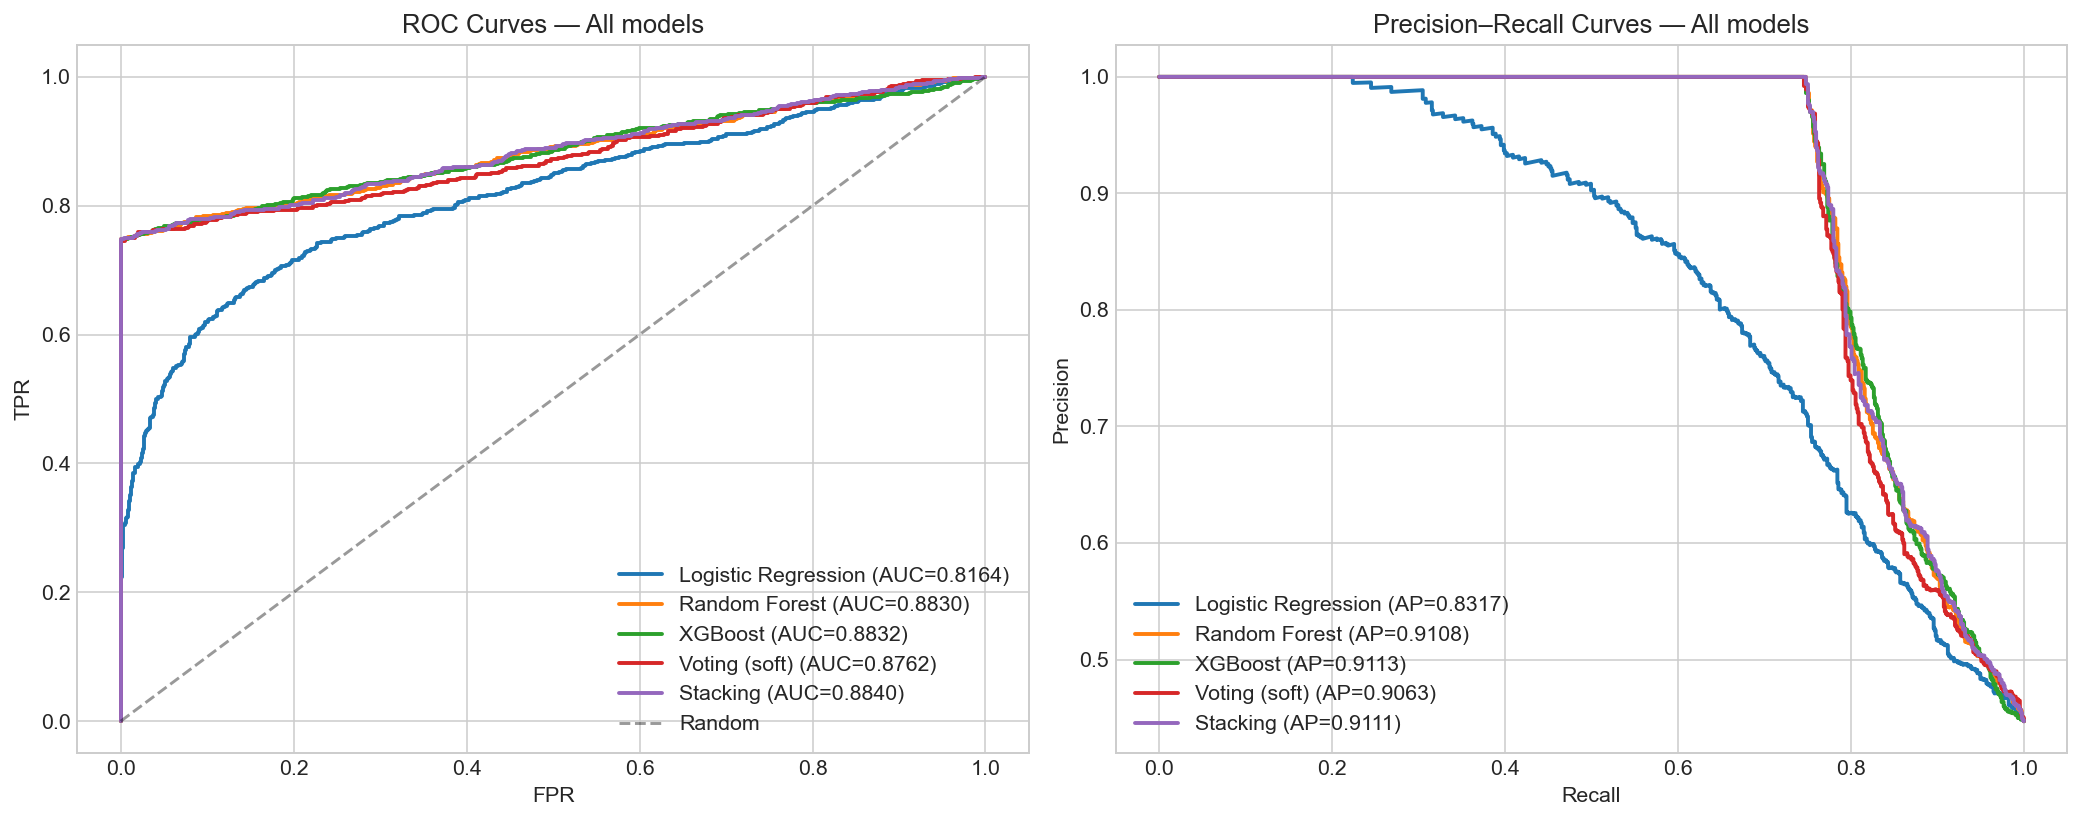
\includegraphics{figures/20_final_roc_pr.png}
\caption{Final ROC and Precision-Recall curves with all models overlaid.
The non-trivial models cluster in a band between F1 = 0.847 and 0.855.}
\end{figure}

Two structural observations come out of this table:

\begin{itemize}
\tightlist
\item
  Every non-trivial model lands within 0.01 F1 of every other one. We
  read this as an empirical case for a feature-set ceiling: with the 22
  processed columns we have, no tuning or architectural change pushes F1
  past \textasciitilde0.855.
\item
  Recall plateaus at 0.745 across every model. All eight of our top
  models miss approximately 25 \% of the attacks. The interpretation we
  ended up with is that those attacks mimic normal sessions in the
  feature space we observe, and no classifier can separate them without
  additional inputs (packet payloads or host-level signals, for
  example).
\end{itemize}

\subsection{Threshold analysis (Figure
21)}\label{threshold-analysis-figure-21}

Because the default 0.5 decision threshold is arbitrary, we swept it on
the XGBoost probabilities and computed F1 for each value.

\begin{figure}
\centering
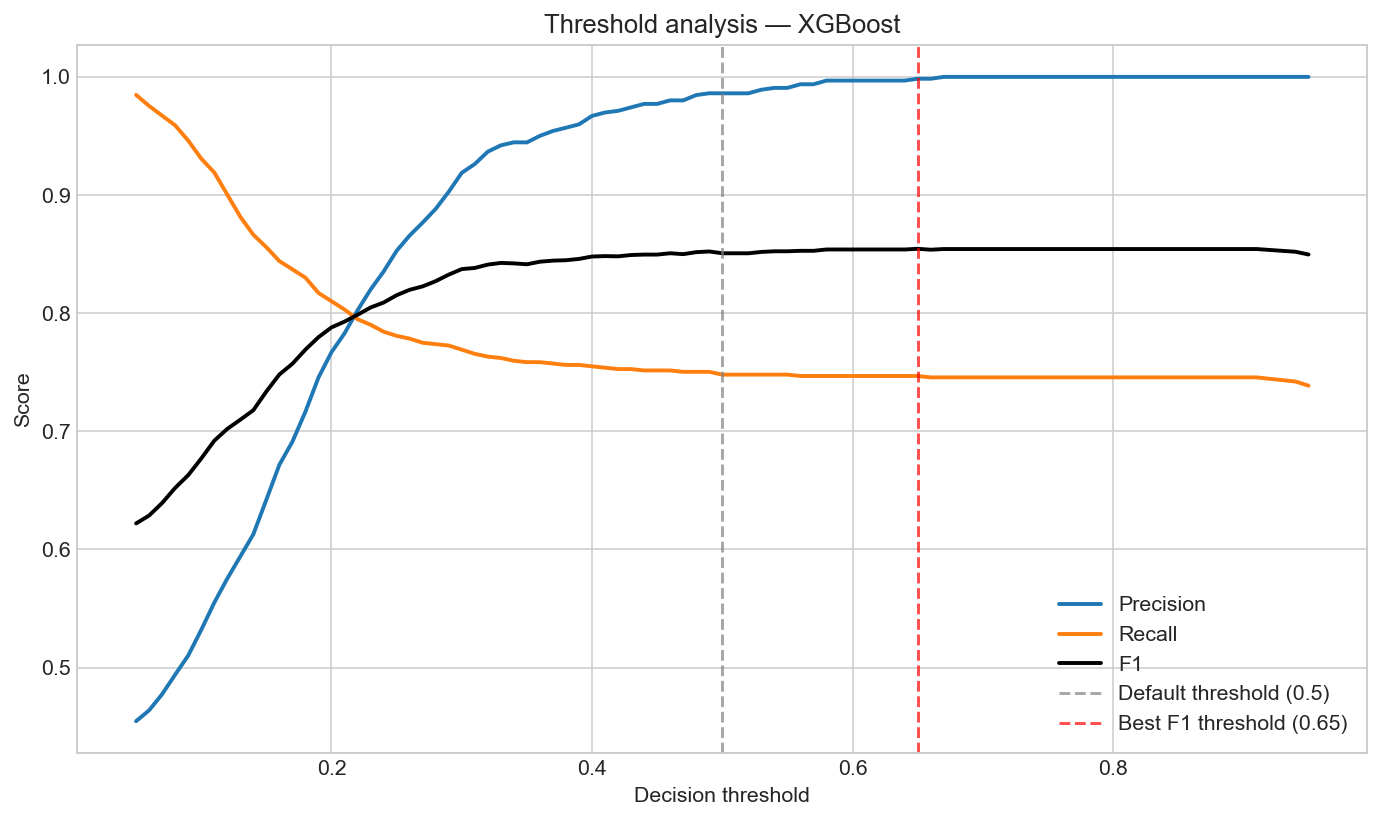
\includegraphics{figures/21_threshold_analysis_xgb.png}
\caption{F1 versus decision threshold for XGBoost. The curve is flat
between 0.4 and 0.75 and peaks at t = 0.65 with F1 = 0.851 --- a
marginal 0.0004 improvement over the default.}
\end{figure}

The F1 curve is essentially flat. It peaks at t = 0.65 with a 0.0004
gain over the default. We kept 0.5 in production because the gain was
not worth the extra parameter to justify, and because the ``what
threshold do you use?'' question is already confusing for newcomers.

\begin{center}\rule{0.5\linewidth}{0.5pt}\end{center}

\section{Interpretability and
Explainability}\label{interpretability-and-explainability}

\subsection{Method choice}\label{method-choice}

We used \textbf{SHAP TreeExplainer} on our tree-based champions (Random
Forest and XGBoost). For the DNN we tried \textbf{KernelExplainer} on a
100-sample background, but the results were too noisy to be useful in
practice, and Tree SHAP was orders of magnitude faster (about 1 ms vs
about 10 s per prediction). Since our champion is Random Forest, Tree
SHAP also happens to be what powers the live explanation in the deployed
UI.

\subsection{Global SHAP (Figures 13, 14,
19)}\label{global-shap-figures-13-14-19}

\begin{figure}
\centering
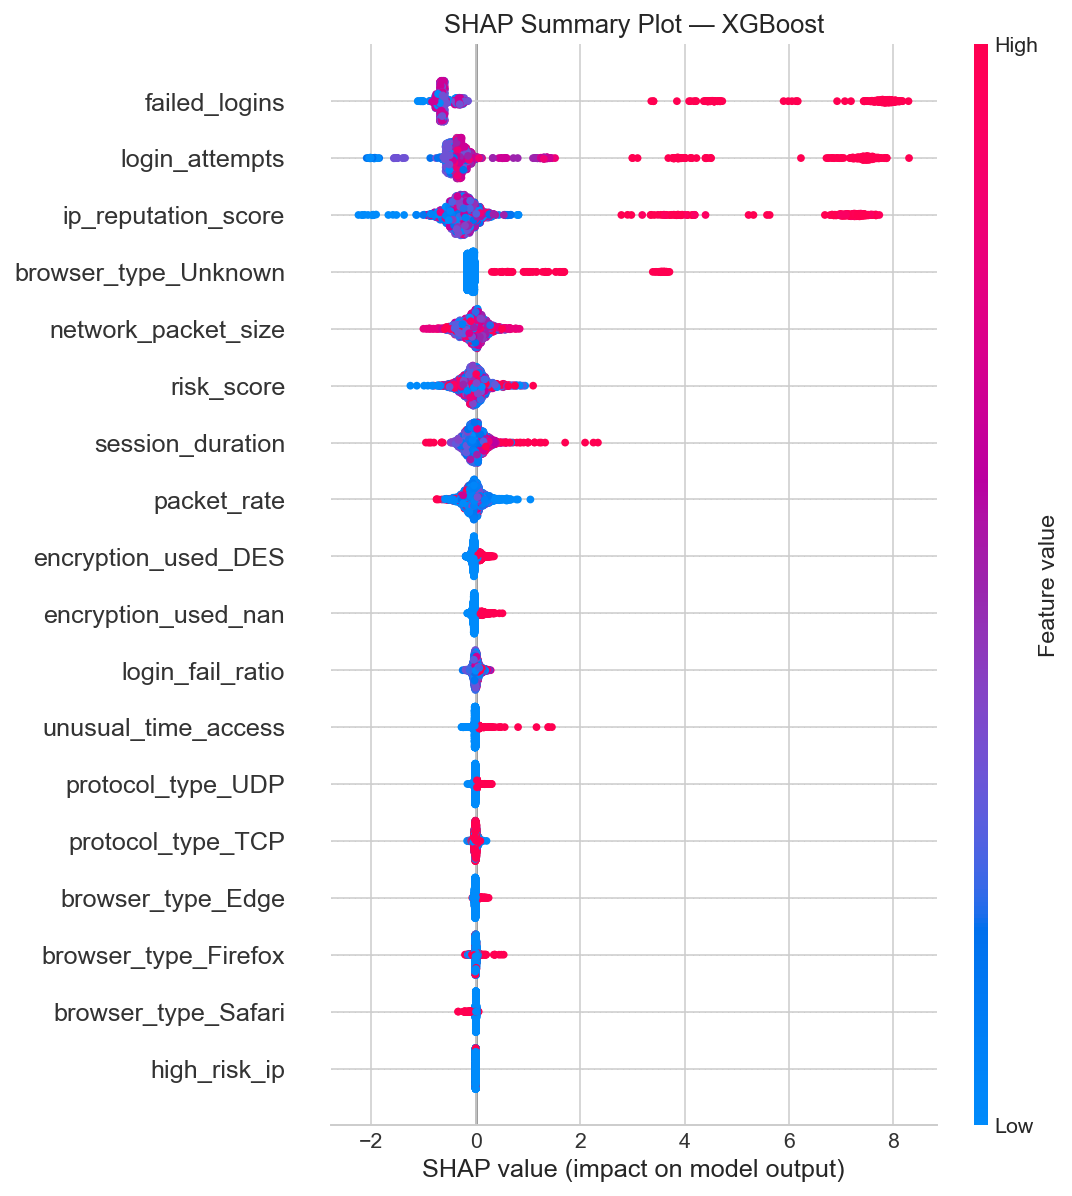
\includegraphics{figures/13_shap_summary_xgb.png}
\caption{SHAP summary plot for XGBoost on the full test set. Points are
samples; the y-axis ranks features by mean \textbar SHAP\textbar; the
x-axis is each feature's contribution to pushing the prediction toward
Attack (right) or Normal (left). Colour is the feature value (red =
high, blue = low).}
\end{figure}

\begin{figure}
\centering
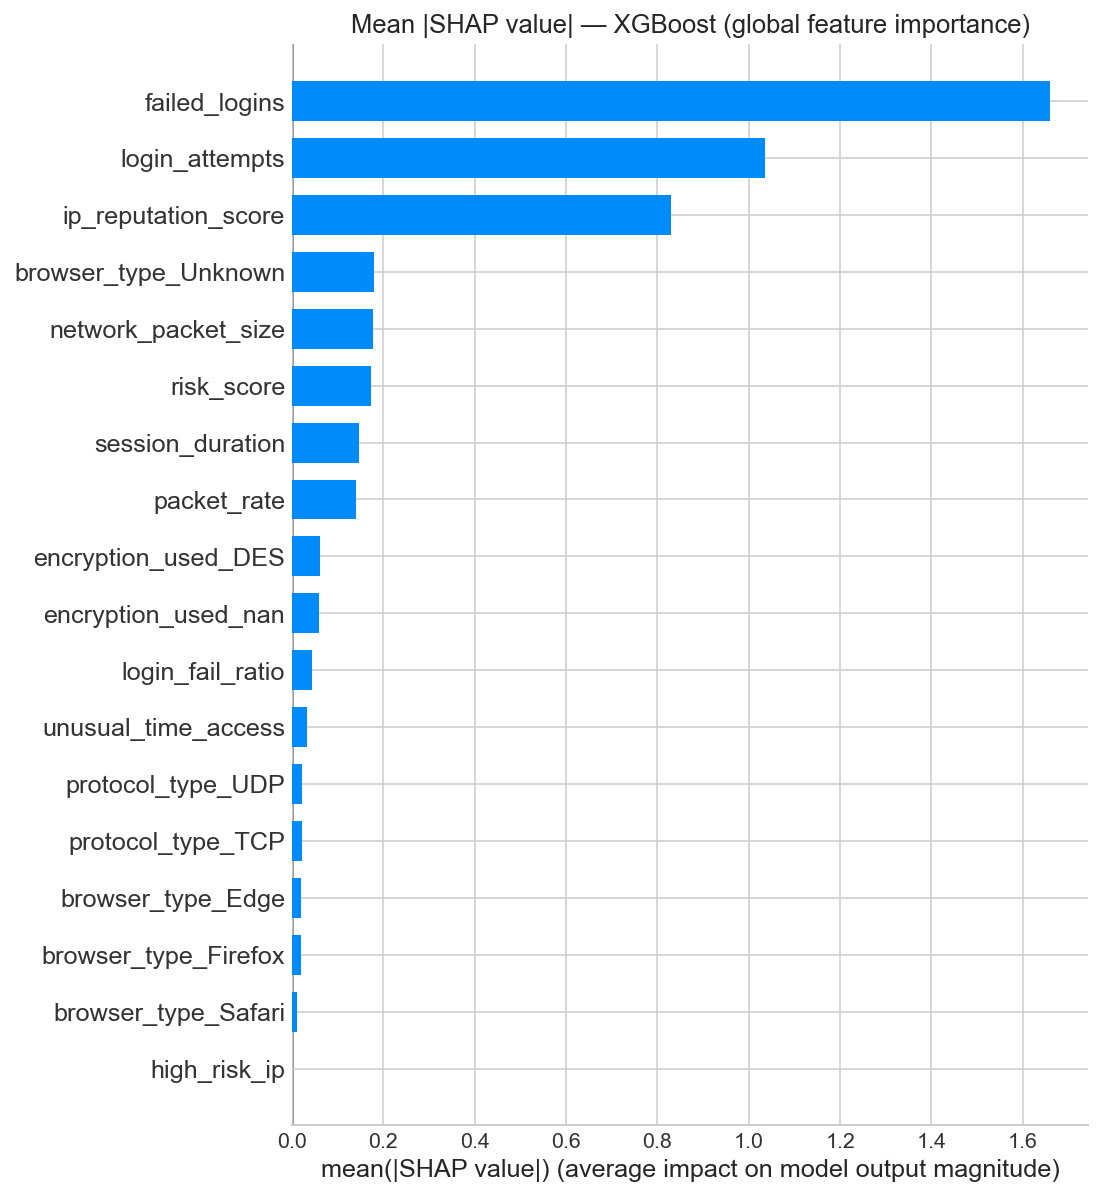
\includegraphics{figures/14_shap_importance_xgb.png}
\caption{Mean absolute SHAP value per feature, XGBoost. failed\_logins
leads at 1.66, followed by login\_attempts (1.03), ip\_reputation\_score
(0.83), then a long tail.}
\end{figure}

\begin{figure}
\centering
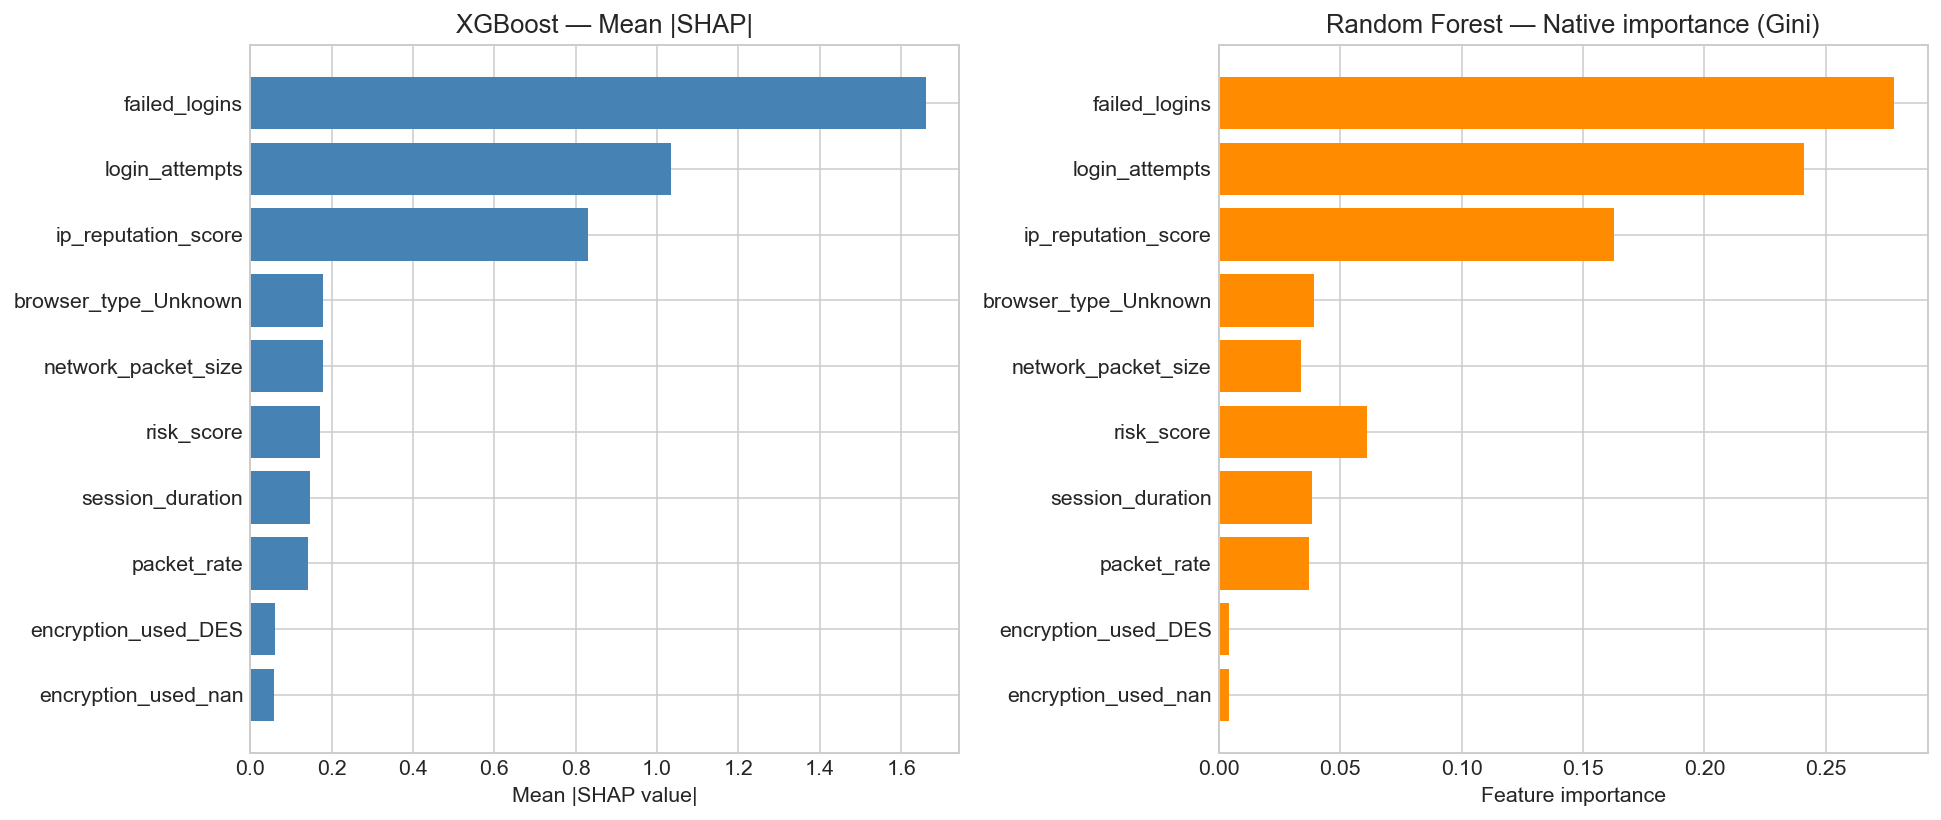
\includegraphics{figures/19_xgb_vs_rf_importance.png}
\caption{Side-by-side comparison of XGBoost SHAP importance and Random
Forest Gini importance. The top three features are identical across
methods, and browser\_type\_Unknown is consistently in the top six for
both.}
\end{figure}

The two tree-based models ranked features almost identically:

\begin{enumerate}
\def\labelenumi{\arabic{enumi}.}
\tightlist
\item
  \texttt{failed\_logins} (mean\textbar SHAP\textbar{} = 1.66 on
  XGBoost; rank 1 on RF Gini)
\item
  \texttt{login\_attempts} (1.03; rank 2)
\item
  \texttt{ip\_reputation\_score} (0.83; rank 3)
\item
  \texttt{browser\_type\_Unknown} (0.18; rank 6 on RF), confirming the
  EDA finding
\item
  \texttt{network\_packet\_size} (0.18; rank 9 on RF). SHAP surfaced it
  higher than Gini did, which suggests it participates mostly through
  interactions.
\end{enumerate}

The convergence between SHAP and Gini told us the explanations were
robust. We were not just looking at an artefact of one specific
importance method.

\subsection{Individual predictions (Figures 15, 16,
17)}\label{individual-predictions-figures-15-16-17}

We picked three representative sessions from the test set (a true
positive, a false positive, and a false negative) and generated SHAP
waterfall plots for each.

\begin{figure}
\centering
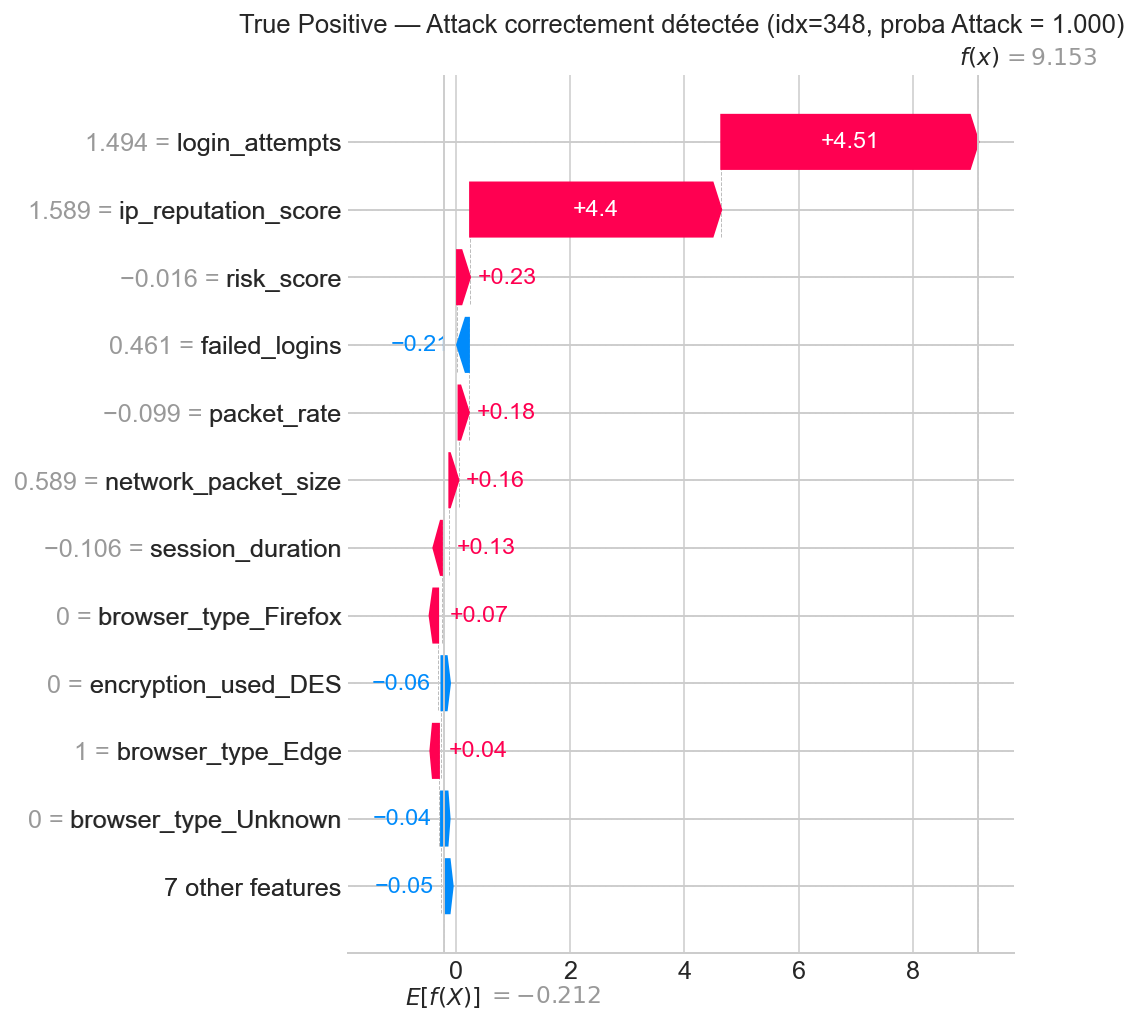
\includegraphics{figures/15_shap_waterfall_tp.png}
\caption{True Positive (idx=348, predicted probability 0.9999). The
attack is obvious: high failed\_logins, browser=Unknown, elevated
ip\_reputation\_score all push toward Attack.}
\end{figure}

\begin{figure}
\centering
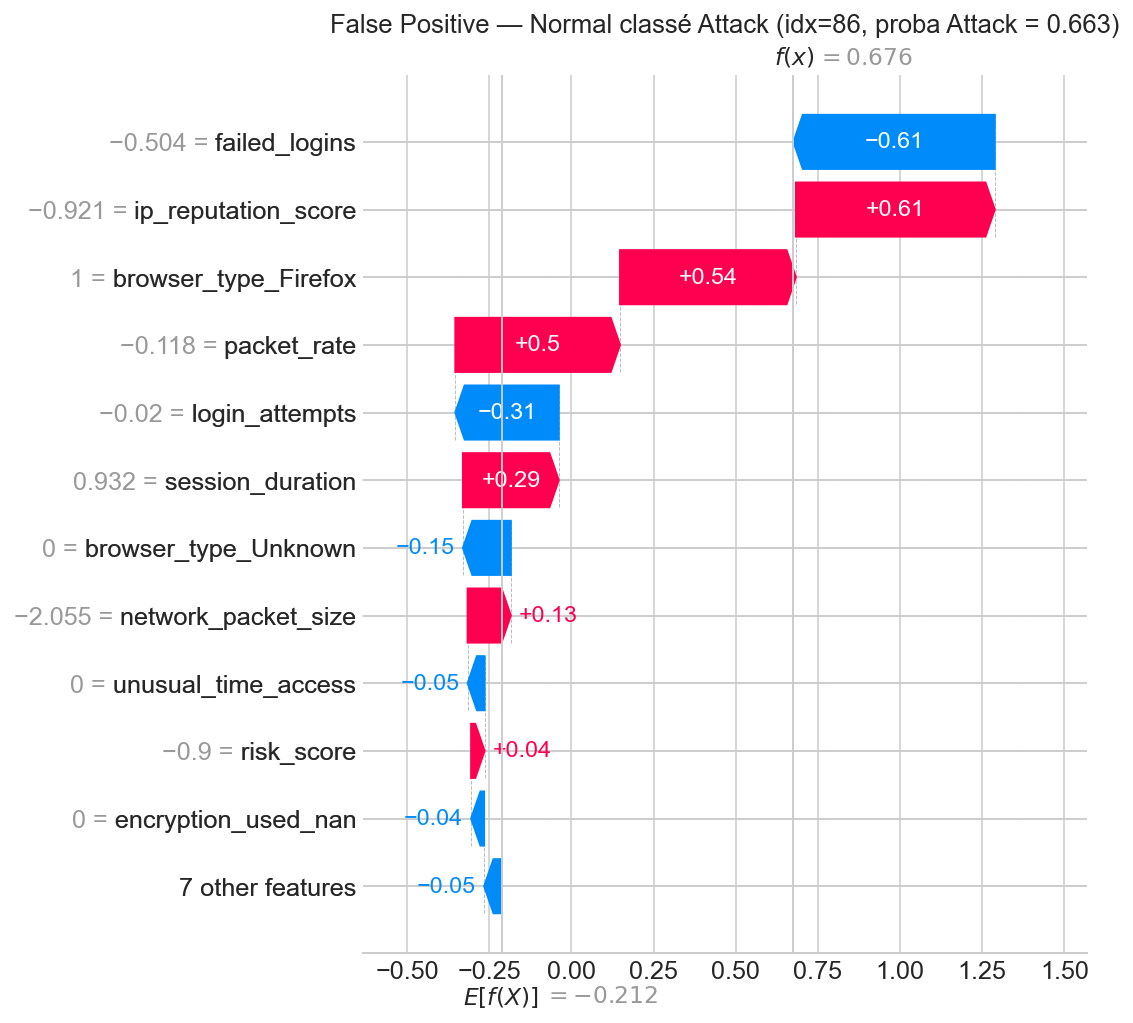
\includegraphics{figures/16_shap_waterfall_fp.png}
\caption{False Positive (idx=86, predicted probability 0.663). The
combination of failed\_logins and browser=Unknown makes the model
over-weight; the session was actually Normal. A clear case where the
model's prior about Unknown browsers is miscalibrated.}
\end{figure}

\begin{figure}
\centering
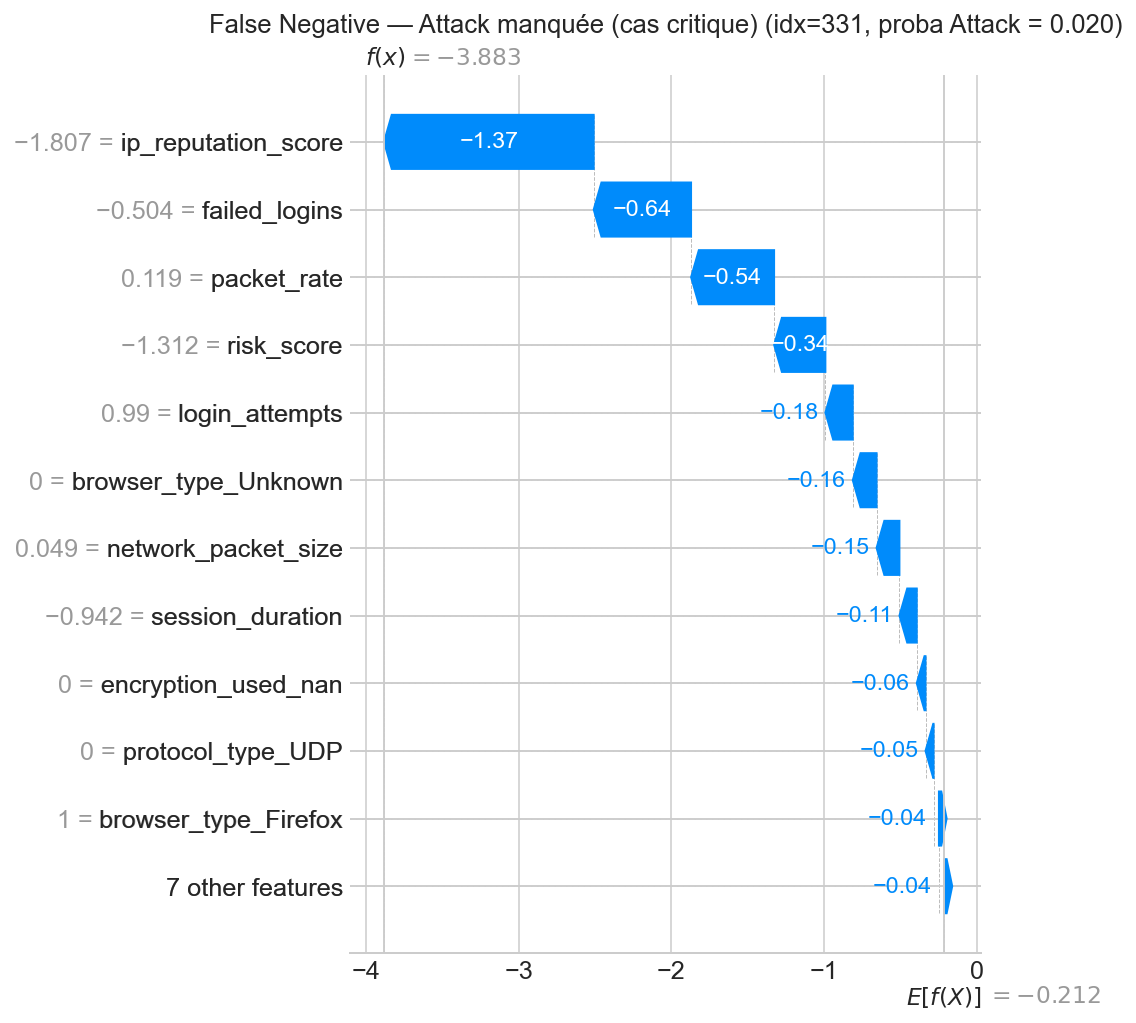
\includegraphics{figures/17_shap_waterfall_fn.png}
\caption{False Negative (idx=331, predicted probability 0.020). An
attack that mimics a normal profile: known browser, encrypted session,
modest login attempts, unremarkable IP reputation. The kind of attack
our feature set cannot catch.}
\end{figure}

The false-negative case deserves special attention. Its features look
entirely typical: Chrome browser, encrypted session, three login
attempts, an IP reputation score of 0.45. Every numerical feature sits
inside the densest part of the Normal distribution. We think attacks of
this kind (an attacker using stolen credentials from a legitimate
endpoint, for instance) are outside the reach of our data, and that no
amount of model tuning would surface them. Detecting them would require
payload inspection or host-level telemetry.

\subsection{Feature dependence (Figure
18)}\label{feature-dependence-figure-18}

\begin{figure}
\centering
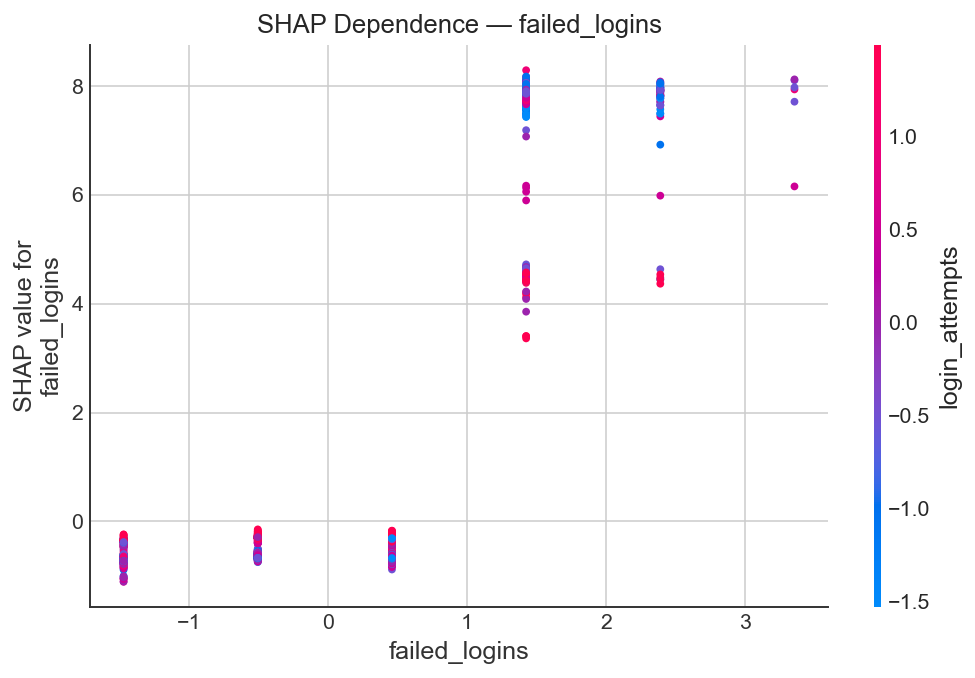
\includegraphics{figures/18_shap_dependence_failed_logins.png}
\caption{SHAP dependence plot for failed\_logins (XGBoost), coloured by
ip\_reputation\_score. The relationship is monotonic: more failed logins
push toward Attack, and the effect is amplified when
ip\_reputation\_score is high.}
\end{figure}

The plot confirms an intuitive interaction: failed logins from a clean
IP are less suspicious than failed logins from a reputation-flagged IP.
Both features contribute independently, and their combination
contributes more than the sum of the parts. That is exactly the kind of
interaction a non-linear model captures and a Logistic Regression
cannot.

\begin{center}\rule{0.5\linewidth}{0.5pt}\end{center}

\section{Deployment and Performance
Tracking}\label{deployment-and-performance-tracking}

\subsection{Architecture}\label{architecture}

We deployed a \textbf{single Docker service},
\texttt{cybersecurity-ids-api}, running on port 8000. The service hosts:

\begin{itemize}
\tightlist
\item
  \texttt{GET\ /health}: Kubernetes-style readiness probe
\item
  \texttt{GET\ /model/info}: model type, path, default threshold,
  training metadata
\item
  \texttt{POST\ /predict}: JSON prediction endpoint
\item
  \texttt{GET\ /} redirects (HTTP 307) to \texttt{/ui}
\item
  \texttt{GET\ /ui}: the Gradio UI mounted on the same FastAPI app via
  \texttt{gr.mount\_gradio\_app(app,\ demo,\ path="/ui")}
\end{itemize}

We chose to use one service instead of one container for the API and one
for the UI, for three reasons. The model stays loaded in memory once.
The UI's prediction calls do not need cross-container HTTP hops. And the
surface of things that can fail to start is halved. MLflow is available
as an optional second service behind \texttt{-\/-profile\ tools}, so
\texttt{docker\ compose\ up\ -d} only launches the evaluated service.

\subsection{Champion bundle and
startup}\label{champion-bundle-and-startup}

At container start, the FastAPI \texttt{startup} event loads
\texttt{saved\_models/best\_model.joblib}. That bundle is a dict
containing the champion model, the fitted preprocessor, the champion
name, the default decision threshold, and training metadata. A second
hook loads the four comparison models (LR, RF, XGBoost, DNN v2) from
\texttt{saved\_models/*.joblib} and \texttt{dnn.weights.h5}. If any of
those is missing, the comparison section of the UI falls back gracefully
to whatever was successfully loaded.

The DNN was saved as \textbf{weights only} (\texttt{dnn.weights.h5})
plus a minimal \texttt{dnn\_arch.joblib} describing
\texttt{n\_features}. The API reconstructs the architecture at load time
and calls \texttt{load\_weights}. We adopted this pattern after running
into a cross-version failure with the \texttt{.keras} format when we
tried to load a host-saved model inside the container.

\subsection{The Gradio UI: live SHAP and 4-model
comparison}\label{the-gradio-ui-live-shap-and-4-model-comparison}

The UI has three parts on one page:

\begin{enumerate}
\def\labelenumi{\arabic{enumi}.}
\tightlist
\item
  A 9-feature input form with sliders, dropdowns, and three one-click
  presets (Normal traffic, Obvious attack, Edge case).
\item
  The champion verdict in a coloured banner: label, probability, and
  risk level (LOW / MEDIUM / HIGH / CRITICAL).
\item
  A SHAP waterfall for the champion's prediction, generated on the fly
  (around 100 ms per call thanks to the cached TreeExplainer). It shows
  the top ten contributing features, with red bars pushing toward Attack
  and blue ones pushing toward Normal.
\item
  A ``All 4 candidate models on this input'' section displaying four
  cards side by side. Each card shows the model's probability on this
  sample, its prediction, its measured inference time, and (below a
  dashed separator) its \textbf{F1 on the full test set}. The best F1 is
  highlighted in green and bold. A banner below the cards reads
  CONSENSUS, PARTIAL, or DISAGREEMENT based on the spread across models,
  and reminds the reader that the champion is chosen on global F1, not
  on the current sample.
\end{enumerate}

This last piece is the core of our demo story. On
\texttt{Obvious\ attack}, all four models cluster around 0.99 to 1.00.
On \texttt{Edge\ case}, Logistic Regression sits at exactly 0.499 (the
linear boundary passes through the sample) while the three non-linear
models all say Normal at 0.13 to 0.18. The live visual makes the
argument of Section 3 tangible in three seconds.

\subsection{\texorpdfstring{\texttt{docker\ compose\ up\ -d} and the
reproducibility
contract}{docker compose up -d and the reproducibility contract}}\label{docker-compose-up--d-and-the-reproducibility-contract}

The full deployment contract is:

\begin{Shaded}
\begin{Highlighting}[]
\BuiltInTok{cd}\NormalTok{ repo/docker}
\ExtensionTok{docker}\NormalTok{ compose up }\AttributeTok{{-}d}
\CommentTok{\# wait \textasciitilde{}7 seconds for the healthcheck to pass}
\CommentTok{\# open http://localhost:8000 in a browser}
\end{Highlighting}
\end{Shaded}

No \texttt{pip\ install}, no model training, no manual file copying.
\texttt{saved\_models/} is committed (three classical \texttt{.joblib},
one \texttt{.h5}, one \texttt{.joblib} arch descriptor, one metadata
file, and one champion bundle), so that \texttt{docker\ compose\ up\ -d}
works from a fresh clone or from the ZIP we submitted, without any
preparatory step.

Two Dockerfile decisions worth mentioning:

\begin{itemize}
\tightlist
\item
  \textbf{Ordered COPY.} \texttt{requirements.txt} is copied before
  \texttt{src/}, so the slow pip install layer (around 3 minutes for
  TensorFlow, XGBoost, SHAP, MLflow, Gradio) is cached when only our
  code changes. This takes the rebuild time from about 3 minutes to
  about 5 seconds for iterative development. We learned this trick the
  hard way after a few painful minutes-long rebuilds.
\item
  \textbf{Read-only model mount.} The container mounts
  \texttt{saved\_models/} as \texttt{:ro} because the API never writes
  model files, and we wanted to keep that path read-only.
\end{itemize}

\subsection{MLflow tracking}\label{mlflow-tracking}

Every training run in notebooks 02, 03 and 05 calls
\texttt{mlflow.start\_run()} inside the \texttt{cybersecurity-ids}
experiment. We logged:

\begin{itemize}
\tightlist
\item
  \textbf{Parameters:} model name, all hyperparameters (stringified to
  avoid non-JSON-serialisable callables in XGBoost), preprocessing
  configuration, random seed
\item
  \textbf{Metrics:} accuracy, precision, recall, F1, ROC-AUC, PR-AUC,
  train time, inference time
\item
  \textbf{Per-epoch metrics for the DNN:} \texttt{loss},
  \texttt{val\_loss}, \texttt{accuracy}, \texttt{val\_accuracy}
\item
  \textbf{Artifacts:} confusion matrix PNG, serialised model
\end{itemize}

This gave us ten runs across the project that we can sort by F1 in the
UI and compare side by side. We deliberately kept MLflow out of the
\texttt{docker\ compose\ up\ -d} default path for two reasons. First,
the evaluation only touches the one service that serves the model.
Second, the run \texttt{meta.yaml} files contain absolute Windows paths
for artefacts, which would not resolve inside a Linux container. MLflow
is available locally via \texttt{mlflow\ ui} from the \texttt{repo/}
directory to inspect the runs.

\begin{center}\rule{0.5\linewidth}{0.5pt}\end{center}

\section{Reflections and
Observations}\label{reflections-and-observations}

\subsection{Challenges faced}\label{challenges-faced}

\begin{itemize}
\item
  \textbf{\texttt{sklearn} cross-version drift broke Logistic Regression
  loading.} The champion bundle was first serialised with
  \texttt{scikit-learn} 1.8.0 on a team member's laptop. The container
  had 1.7.2. Random Forest unpickled with a warning but ran fine.
  Logistic Regression raised
  \texttt{AttributeError:\ \textquotesingle{}LogisticRegression\textquotesingle{}\ object\ has\ no\ attribute\ \textquotesingle{}multi\_class\textquotesingle{}}
  because the attribute had been removed in 1.8. We pinned
  \texttt{scikit-learn==1.7.2} in \texttt{requirements.txt} and
  retrained every model in that environment. The incident cost us about
  an hour and taught us that ``warnings we ignored'' in the notebook
  were hiding a real inference-time failure.
\item
  \textbf{\texttt{.keras} model format failed to deserialise
  cross-version.} The DNN, saved with \texttt{tf.keras} on the host,
  refused to load inside the container with an error about an
  unrecognised \texttt{quantization\_config} argument on \texttt{Dense}
  layers. The container and host both had TensorFlow 2.21.0, but the
  Keras internal serialisation format had evolved between minor
  versions. We switched to weights-only (\texttt{dnn.weights.h5}) plus a
  tiny architecture descriptor, and we now rebuild the model in-place at
  load time. This was the most portable way we found to ship a Keras
  model across environments.
\item
  \textbf{MLflow \texttt{meta.yaml} files carry absolute paths.} When we
  tried to spin up the MLflow UI inside Docker to show the runs live, we
  noticed that every run recorded
  \texttt{artifact\_uri:\ file:C:\textbackslash{}Users\textbackslash{}...\textbackslash{}mlruns\textbackslash{}...},
  which does not exist in a Linux container. The UI would list the runs
  and metrics but fail on the artefact preview. We moved MLflow to an
  optional profile and recommended running \texttt{mlflow\ ui} directly
  on the host for inspection.
\item
  \textbf{Gradio 6 deprecated \texttt{theme=} on the \texttt{Blocks}
  constructor.} A minor warning, harmless in practice but noisy at
  startup. We left it as-is. Moving theme to \texttt{launch()} would
  have forced us to un-mount from FastAPI.
\end{itemize}

\subsection{Key takeaways}\label{key-takeaways}

\begin{itemize}
\tightlist
\item
  \textbf{Stop tuning when you hit a plateau, look at the data instead.}
  Once every non-trivial model landed within 0.01 F1 of the others, we
  stopped tweaking hyperparameters and started looking at the recall
  ceiling itself. Reporting \emph{why} the metric plateaus at 0.745 is a
  more useful contribution than a 0.001 F1 improvement from another
  GridSearchCV sweep.
\item
  \textbf{Engineered features earn their place or they do not.} Three of
  our four engineered features ranked in the top six by correlation with
  the target. \texttt{packet\_rate} did not. We kept it anyway because
  it is cheap to compute and a tree model can still exploit it through
  interactions.
\item
  \textbf{Trees beat DL on tabular data of this size.} We trained 4 DNN
  variants with proper regularisation, and none of them matched Random
  Forest. This is consistent with the recent literature
  (\href{https://arxiv.org/abs/2207.08815}{Grinsztajn et al.~2022}) and
  with common experience. DL shines on unstructured data (images, audio,
  text) where automatic feature extraction is the whole value
  proposition. On a 22-column tabular problem with engineered features
  that already do the heavy lifting, a gradient-boosted or bagged
  ensemble is the right tool.
\item
  \textbf{Interpretability belongs in the deployed product.} A SHAP
  waterfall that shows up \emph{inside the prediction UI} makes the
  explainability argument every time a user clicks Predict. A SHAP
  summary plot in a static report is a one-off the reader forgets.
\item
  \textbf{The cost of a feature is also what it adds to the demo story.}
  Our 4-model comparison costs us about 300 ms per prediction and two
  extra model loads at startup. It is not the highest-performing
  addition we could have made. But it lets us defend our champion choice
  in the UI without any slide. The demo user sees \emph{live} that every
  non-trivial model converges to about 0.85 F1 on the full test set, and
  that the champion is just the best one in a close race.
\end{itemize}

\subsection{Limits and future work}\label{limits-and-future-work}

\begin{itemize}
\tightlist
\item
  \textbf{Recall ceiling of 0.745 is fundamental, not algorithmic.}
  Lifting it would require new inputs (packet payload features, host
  telemetry, or temporal context such as session sequences). Anything we
  could have tried on the existing features would be inside the noise.
\item
  \textbf{The Unknown-browser prior can misfire.} Figure 16 (false
  positive) shows a Normal session flagged Attack because of a
  combination of browser=Unknown and elevated failed\_logins. A
  threshold adjustment or a second-stage classifier that explicitly
  re-evaluates Unknown cases could raise precision further, at a small
  cost to recall.
\item
  \textbf{Continuous retraining.} The MLflow + Docker setup we built is
  already the infrastructure for a retraining pipeline. A cron job that
  re-runs \texttt{scripts/export\_models.py} on fresh data would produce
  a new bundle, and the API would pick up the new bundle on restart with
  no code change. We did not wire the cron job, but everything else is
  in place.
\item
  \textbf{Explainability for the DNN.} We used KernelExplainer and found
  it too slow to be useful in a UI. DeepExplainer would be a faster
  alternative to try, at the cost of a TF dependency in production. With
  Random Forest as the champion, this is a ``nice to have'', not a
  blocker.
\end{itemize}

\begin{center}\rule{0.5\linewidth}{0.5pt}\end{center}

\section{Conclusion}\label{conclusion}

We set out to build an interpretable, deployable intrusion detection
model. The final deliverable is closer to ``defensible'' than
``best-in-class'', and we think that is the right mode for this problem
and this data. The dataset's feature set imposes a performance ceiling
around F1 = 0.855 and recall = 0.745, and within that ceiling all four
of our non-trivial models converge to the same place. We deployed the
one that was fastest and simplest to serve, backed the choice with four
candidate models running side by side in the UI, and made every
prediction self-explanatory with a live SHAP waterfall. The full project
launches with \texttt{docker\ compose\ up\ -d} and opens at
\texttt{http://localhost:8000}.

Beyond the F1 number, the part of the project we would want to highlight
is the reasoning around why it plateaus where it does, and the UI that
surfaces that reasoning on every click.

\begin{center}\rule{0.5\linewidth}{0.5pt}\end{center}

\emph{Project files submitted in this ZIP:}
\texttt{repo/notebooks/01–05} (EDA through final comparison),
\texttt{repo/src/} (pipeline modules, FastAPI service, Gradio UI),
\texttt{repo/scripts/export\_models.py} (reproducible training),
\texttt{repo/saved\_models/} (pre-fitted artefacts),
\texttt{repo/docker/} (Dockerfile + docker-compose.yml),
\texttt{repo/reports/figures/} (21 figures plus confusion matrices),
\texttt{repo/README.md}, \texttt{repo/requirements.txt}.
